\documentclass{article}


\usepackage{PRIMEarxiv}

\usepackage[utf8]{inputenc} % allow utf-8 input
\usepackage[T1]{fontenc}    % use 8-bit T1 fonts
%\usepackage{hyperref}       % hyperlinks
\usepackage{url}            % simple URL typesetting
\usepackage{booktabs}       % professional-quality tables
\usepackage{amsfonts}       % blackboard math symbols
\usepackage{nicefrac}       % compact symbols for 1/2, etc.
\usepackage{microtype}      % microtypography
\usepackage{lipsum}
%\usepackage{fancyhdr}       % header
\usepackage{graphicx}       % graphics
\graphicspath{{media/}}     % organize your images and other figures under media/ folder

\usepackage{xcolor}  % For more color options
\usepackage[colorlinks=true, allcolors=blue]{hyperref}
\usepackage{amsmath}
\usepackage{amsthm}
\usepackage{amssymb}
\usepackage{mathtools}
\usepackage{stmaryrd}
\usepackage[ruled,lined,linesnumbered,boxed]{algorithm2e}
\usepackage{bbm}
\usepackage{multirow}
%\usepackage{natbib} % Added natbib package
\usepackage[square,authoryear]{natbib}
% Redefine \citet to use parentheses instead of brackets
%\setcitestyle{square} % For \citep
%\setcitestyle{round,aysep={}}
% Custom formatting to move the caption below the algorithm
%\makeatletter
%\renewcommand{\@algocf@capt@plain}{bottom}
%\makeatother

%Header
\pagestyle{fancy}
\thispagestyle{empty}
\rhead{ \textit{ }}

% Update your Headers here
%\fancyhead[LO]{Running Title for Header}
\fancyhead[LO]{}
% \fancyhead[RE]{Firstauthor and Secondauthor} % Firstauthor et al. if more than 2 - must use \documentclass[twoside]{article}


%% Title
\title{Optimal Certified Radius Estimation in Randomized Smoothing
%%%% Cite as
%%%% Update your official citation here when published 
\thanks{
Last updated on \today.}
}

\author{
    Zakariae MOUTAOUAKIL\\
%    Affiliation \\
    Paris Cité University\\
%    City\\
    Zakariae.moutaouakil@etu.u-paris.fr\\
%% examples of more authors
%    \And
%    Author3 \\
%    Affiliation \\
%    Univ \\
%    City\\
%    \texttt{email@email} \\
%% \AND
%% Coauthor \\
%% Affiliation \\
%% Address \\
%% \texttt{email} \\
%% \And
%% Coauthor \\
%% Affiliation \\
%% Address \\
%% \texttt{email} \\
%% \And
%% Coauthor \\
%% Affiliation \\
%% Address \\
%% \texttt{email} \\
}

\sloppy
\newtheorem{proposition}{Proposition}
\newtheorem{lemma}{Lemma}
\DeclareMathOperator*{\argmax}{arg\,max}


\begin{document}
    \maketitle

    \begin{abstract}
    Randomized smoothing has emerged as a promising technique for certifying the robustness of machine learning models against adversarial perturbations.
    However, current methods for estimating the certified radius and, consequently, the certified test-set accuracy often suffer from overly pessimistic conservativeness.
    This paper introduces a novel approach to improve the estimation of certified radii, leading to tighter bounds on certified test-set accuracy.
    Our method makes use of advanced statistical and optimization techniques to estimate the certified radius in an optimal manner.
    Extensive experiments on the CIFAR-10 and ImageNet datasets demonstrate the efficacy of our method.

%    \textbf{Keywords:} adversarial robustness, randomized smoothing, certified radius, test-set accuracy, CIFAR-10, ImageNet
\end{abstract}

\keywords{adversarial robustness \and randomized smoothing \and certified radius \and test-set accuracy \and CIFAR-10 \and ImageNet}
% keywords can be removed
%\keywords{First keyword \and Second keyword \and More}


    \section{Introduction}\label{sec:introduction}
The rapid advancement of deep neural networks has revolutionized numerous fields, from computer vision~\citep{krizhevsky2012imagenet} to natural language processing~\citep{devlin2018bert}.
These powerful models have demonstrated an unprecedented ability to learn complex patterns from data, leading to remarkable performance in a wide array of tasks~\citep{lecun2015deep}.
As deep learning continues to permeate various aspects of our lives, from smartphone applications to autonomous vehicles, the integration of these models into critical systems has become increasingly commonplace~\citep{goodfellow2016deep}.

However, this widespread adoption has brought to light significant concerns regarding the security and reliability of neural networks~\citep{biggio2018wild}.
As these models become more deeply embedded in our technological infrastructure, addressing their vulnerabilities has become a matter of paramount importance.
The field of adversarial machine learning has emerged as a crucial area of research, focusing on understanding and mitigating the susceptibility of neural networks to malicious attacks~\citep{vorobeychik2018adversarial}.

One of the primary challenges in neural network security is adversarial robustness~\citep{szegedy2013intriguing}.
Adversarial examples, which are imperceptibly perturbed inputs designed to fool state-of-the-art models, have been shown to pose significant threats to deployed systems~\citep{goodfellow2014explaining}.
These vulnerabilities have been demonstrated across various domains, including image classification~\citep{carlini2017towards}, speech recognition~\citep{carlini2018audio}, and even physical-world applications~\citep{kurakin2016adversarial}.
The ease with which these adversarial examples can be generated and their transferability across different models have raised serious concerns about the reliability of neural networks in security-sensitive applications~\citep{papernot2016transferability}.

The implications of such vulnerabilities extend far beyond academic interest.
In safety-critical applications like autonomous vehicles~\citep{eykholt2018robust} or medical diagnosis systems~\citep{finlayson2019adversarial}, adversarial attacks could lead to catastrophic consequences.
For instance, subtle perturbations to road signs could cause an autonomous vehicle to misinterpret critical signals, potentially leading to accidents.
Similarly, in healthcare, adversarial manipulations of medical images could result in misdiagnosis, putting patients' lives at risk.
Moreover, as machine learning models become more prevalent in security-sensitive areas such as malware detection~\citep{grosse2017adversarial} and biometric authentication~\citep{sharif2016accessorize}, the potential for malicious exploitation grows exponentially.

The financial sector is another domain where the security of neural networks is of utmost importance.
Machine learning models are increasingly being used for fraud detection, credit scoring, and algorithmic trading~\citep{gu2018adversarial}.
Adversarial attacks in these contexts could lead to significant financial losses and erode trust in financial institutions.
The potential for market manipulation through adversarial techniques poses a serious threat to the stability of financial systems~\citep{li2020adversarial}.

Efforts to address these security challenges have given rise to a burgeoning field of research focused on developing robust machine learning models~\citep{madry2017towards}.
Defensive strategies range from adversarial training~\citep{tramer2017ensemble} to input preprocessing techniques~\citep{guo2017countering} and detection methods~\citep{metzen2017detecting}.
Adversarial training, which involves augmenting the training data with adversarial examples, has shown promise in improving model robustness.
However, this approach often comes at the cost of increased computational complexity and potential degradation of performance on clean data~\citep{tsipras2018robustness}.
Input preprocessing techniques aim to remove adversarial perturbations before feeding the data into the neural network.
These methods include various image transformations, such as bit-depth reduction, JPEG compression, and total variation minimization~\citep{xu2017feature}.
While these approaches can be effective against certain types of attacks, they often struggle to generalize to more sophisticated adversarial perturbations.

Detection methods, on the other hand, focus on identifying adversarial examples at test time.
These approaches leverage various statistical properties of adversarial examples or employ separate neural networks trained to distinguish between clean and adversarial inputs~\citep{meng2017magnet}.
However, many of these detection methods have been shown to be vulnerable to adaptive attacks, where the adversary is aware of the defense mechanism and can craft adversarial examples that evade detection~\citep{athalye2018obfuscated}.

The limitations of these empirical defense strategies have highlighted the need for more principled approaches to neural network security.
In response to these challenges, recent years have seen a growing interest in certifiable robustness guarantees for neural networks~\citep{cohen2019certified}.
These approaches aim to provide formal assurances about a model's behavior under bounded perturbations, offering a rigorous foundation for building secure AI systems.
Certifiable robustness techniques can be broadly categorized into two main approaches: exact methods and relaxation-based methods.
Exact methods, such as Mixed Integer Linear Programming (MILP)~\citep{tjeng2017evaluating} and Satisfiability Modulo Theories (SMT)~\citep{katz2017reluplex}, provide precise robustness guarantees but are computationally expensive and scale poorly to large neural networks.
Relaxation-based methods, on the other hand, offer more scalable solutions by approximating the network's behavior.
These include techniques based on abstract interpretation~\citep{gehr2018ai2}, semidefinite programming~\citep{raghunathan2018semidefinite}, and linear programming~\citep{wong2018provable}.

While these certifiable robustness techniques have made significant progress, they often struggle to scale to state-of-the-art neural network architectures and typically provide overly conservative bounds.
This has led to a growing interest in probabilistic certification methods, which offer a balance between scalability and rigorous guarantees.
Among these probabilistic certification methods, randomized smoothing has emerged as a particularly promising technique for achieving scalable and flexible robustness certification~\citep{cohen2019certified}.
This approach involves adding random noise to the input and using the probabilistic properties of the smoothed classifier to derive robustness guarantees.
Randomized smoothing has gained significant attention due to its ability to scale to large neural networks and its applicability to various types of data and model architectures.

As we continue to rely more heavily on deep learning systems in critical applications, the importance of addressing their security vulnerabilities cannot be overstated.
The field of adversarial machine learning is rapidly evolving, with new attack methods and defense strategies constantly emerging.
While significant progress has been made in understanding and mitigating these vulnerabilities, many challenges remain.

The development of robust and secure neural networks requires a multifaceted approach, combining empirical defenses, formal verification techniques, and novel architectural designs.
As we move forward, it is crucial to not only focus on defending against known attack methods but also to anticipate and prepare for future threats.
This necessitates a proactive approach to security, integrating robustness considerations into the very foundations of neural network design and training.
In the following sections, we will delve deeper into the concept of randomized smoothing, exploring its theoretical foundations, practical implementations, and its certifiable robustness guarantees for neural networks.

In summary, this paper is structured as follows:
\begin{itemize}
    \item Section~\ref{sec:background-&-related-work} presents the theoretical foundations of randomized smoothing, alongside notations and definitions we will use throughout the paper.
    \item Section~\ref{sec:problem-formulation} defines precisely the problem we will address in this paper, and divides into two subproblems: the discrete case and the continuous case.
    \item Our contributions start at section~\ref{sec:discrete}, where we tackle the discrete case first.
    \item Section~\ref{sec:continuous} starts with a presentation of a new type of confidence intervals in subsection~\ref{subsec:estimating-by-betting}.
    The rest of the section formulates our contribution for the continuous case.
    \item Section~\ref{sec:experiments} validates our theoretical results on real-world datasets, such as CIFAR-10 and ImageNet.
\end{itemize}

    \section{Background \& Related Work}\label{sec:background-&-related-work}

\subsection{Notation}\label{subsec:notation}
Let $\mathcal{X}$ be a subset of the input space $\mathbb{R}^d$.
We identify the set of labels $\mathcal{Y}$ with the set of integers $\{1, \ldots, m\}$, where $m$ is the number of classes.

If $x$ is a data point in $\mathcal{X}$ and $y$ is its true label in $\mathcal{Y}$, then the prediction of a typical neural network classifier $F_{out}: \mathcal{X} \rightarrow \mathcal{Y}$ can be decomposed as $F_{out}(x)=\arg\max_{k \in \mathcal{Y}}s_k\circ f(x)$ where $g: \mathcal{X} \rightarrow \mathbb{R}^m$ is a subclassifier that outputs logits
and $s: \mathbb{R}^m \rightarrow \Delta^{m-1}$ is the normalizing last layer that projects onto the $(m-1)$-dimensional probability simplex defined as:
\[
    \Delta^{m-1} \coloneqq \left\{p \in \mathbb{R}^m : \, p_i \geq 0, \,\sum_{i=1}^m p_i = 1 \right\}.
\]

We denote by $F\coloneqq s\circ f$ the classifier that outputs a probability distribution over the $m$ classes.
We call $F$ the \textbf{soft classifier}, and $F_{out}$ the \textbf{hard classifier}.

The simplex maps that are most commonly found in the literature are the softmax~\citep{bridle1989training}, the hardmax that is defined as the projection that puts all mass in the index of the maximum component (with ties broken arbitrarily), and the sparsemax~\citep{martins16} that is defined as the Hilbert projection onto the convex closed set which is the $(m-1)$-dimensional probability simplex.

We will call the case where we use the hardmax as a simplex map the \textbf{discrete case} and the case where we use a continuous simplex projection (like the softmax or the sparsemax) the \textbf{continuous case}.

\subsection{Randomized Smoothing}\label{subsec:randomized-smoothing}
Randomized smoothing is a technique designed to enhance the robustness of classifiers against small perturbations or adversarial attacks that stems from a simple intuition: if a classifier's decision is stable under small random perturbations of the input, it's likely to be more robust overall (this intuition will be made more rigorous using the concept of robustness radius in section~\ref{subsec:robustness-radius}).

Figure~\ref{fig:pandas} from~\citep{cohen2019certified} provides a visual representation of how randomized smoothing works in practice.
The left image shows an original input $x$ - in this case, a clear photograph of a panda.
The right image demonstrates the effect of applying Gaussian noise with $\sigma = 0.5$ to the same input.
This noisy version represents one of the many perturbations over which the smoothed classifier makes its prediction.
\begin{figure}[htbp]
    \centering
    \includegraphics[width=0.8\textwidth]{images/pandas}
    \caption{Visualization of randomized smoothing. Left: Original input image $x$ of a giant panda. Right: The same image with Gaussian noise applied ($\sigma = 0.5$), illustrating the concept of randomized smoothing. The smoothed classifier's prediction is based on the most likely prediction by the base classifier on such random Gaussian corruptions of $x$. Note that this Gaussian noise is much larger in magnitude than typical adversarial perturbations, helping to "drown out" smaller adversarial attacks and improve classifier robustness.}
    \label{fig:pandas}
\end{figure}

Importantly, the magnitude of this Gaussian noise is much larger than typical adversarial perturbations.
This illustrates a key intuition behind randomized smoothing: by considering predictions over these large random perturbations, the classifier becomes robust to smaller, potentially adversarial changes in the input.
In essence, the large random perturbations ``drown out'' the smaller adversarial ones.

With this visual intuition in mind, we can formally define the smoothed classifier.
Following the same conventions in the previous section, we define the smoothed classifier $\hat{F}: \mathcal{X} \rightarrow \Delta^{m-1}$ using randomized smoothing as implementing a majority vote over predictions of the soft classifier $F$ with noisy versions of the input:

\begin{align*}
    \hat{F}(x) \coloneqq \mathbb{E}_{\epsilon \sim \mathcal{N}(0, \sigma^2 I)} [F(x + \epsilon)],
\end{align*}

where $\epsilon \sim \mathcal{N}(0, \sigma^2 I)$ represents isotropic Gaussian noise with mean $0$ and covariance matrix $\sigma^2 I$.
The final smoothed classifier is given by $\hat{F}_{out}(x) = \arg\max_{k \in \mathcal{Y}} \hat{F}_k(x)$.
We can reinterpret this expectation as convolving $F$ with the Gaussian kernel $p_\sigma$; $\hat{F} = F * p_\sigma$, where
\begin{align*}
    p_\sigma(z) \coloneqq \frac{1}{(2\pi\sigma^2)^{d/2}} \exp\left(-\frac{\|z\|^2}{2\sigma^2}\right).
\end{align*}

\subsection{Robustness Radius}\label{subsec:robustness-radius}

For a given classifier $F: \mathcal{X} \rightarrow \Delta^{m-1}$, we can quantify its decision confidence for a specific input $x$ using a metric called the \textit{certified radius}, denoted as $R(F,x)$.
This radius represents the maximum allowable perturbation $\epsilon$ that can be applied to the input $x$ while ensuring the classifier's output remains consistent with the true label $y$.

The certified radius serves as an indicator of a classifier's resilience to input disturbances.
A larger value of $R(F,x)$ suggests greater robustness against perturbations for that particular input.

Figure~\ref{fig:radius} illustrates this concept visually.
The left panel shows a 2D projection of the decision boundaries of a smoothed classifier.
The concentric dashed circles represent different perturbation radii around an input point $x$.
The right panel shows the probabilities assigned to different classes (represented by colors) as the perturbation radius increases.
\begin{figure}[htbp]
    \centering
    \includegraphics[width=0.8\textwidth]{images/radius}
    \caption{Visualization of randomized smoothing and robustness radius. Left: 2D projection of decision boundaries for a smoothed classifier, with concentric circles representing increasing perturbation radii around input point x. Colors indicate different class regions. Right: Bar chart showing how class probabilities (represented by colored bars) change as perturbation radius increases. $\underline{p_A}$ and $\overline{p_B}$ denote pessimistic bounds on the probabilities of the top two classes at a given radius. This illustration demonstrates how the certified radius is determined as the largest perturbation within which the original class maintains the highest probability.}
    \label{fig:radius}
\end{figure}

The certified radius $R(F,x)$ would correspond to the largest circle in the left panel where the original class (blue in this case) maintains the highest probability.
In the right panel, this would be the point where the blue bar remains the tallest.

In the context of randomized smoothing with Gaussian noise, the size of the perturbation is usually measured using the $\ell_2$-norm, therefore we can formally define the certified radius as:

\begin{align*}
    R(F,x) \coloneqq
    \begin{cases}
        0 & \text{if } F_{out}(x) \neq y, \\[2ex]
        \min \left\{ \epsilon > 0 \,|\, \exists \tau \in B_2(0,\epsilon),\, F_{out}(x + \tau) \neq y \right\} & \text{otherwise,}
    \end{cases}
\end{align*}

where $B_2(0,\epsilon)$ represents the $\ell_2$-ball centered at the origin with radius $\epsilon$.

\subsection{Certified Radius and Lipschitz Constant}\label{subsec:certified-radius-and-lipschitz-constant}

The concept of Lipschitz continuity provides an intuitive framework for understanding classifier robustness and its relation to the certified radius.

A soft classifier $F: \mathcal{X} \rightarrow \Delta^{m-1}$ is \textit{Lipschitz continuous} if there exists a constant $L \geq 0$ such that for all $x_1, x_2 \in \mathcal{X}$:
\begin{align*}
    \lVert F(x_1)- F(x_2) \rVert \leq L \cdot \lVert  x_1- x_2\rVert.
\end{align*}
Lipschitz continuity essentially bounds the maximum change in the output for a given change in the input, which means that a smaller Lipschitz constant indicates that the classifier's output is less sensitive to input perturbations.

The following proposition highlights the relationship between Lipschitz continuity and a quantity named the \textit{prediction margin} $M(F,x)$ (defined below) which quantifies how far the input is from the decision boundary of the classifier.
A positive margin indicates correct classification, with larger values suggesting higher confidence, while a negative margin indicates misclassification:
\begin{equation}
    M(F,x) \coloneqq F(x)_{y} - \max_{i \neq y}\{F(x)_i\}.\label{eq:prediction-margin}
\end{equation}
\begin{proposition}[\citep{tsuzuku2018lipschitz}]
    If the classifier $F$ is Lipschitz continuous with Lipschitz constant $L(F)$ and if $M(F,x)>\sqrt{2}L(F)r$, then for any adversarial example $x+\epsilon$ such that $\lVert \epsilon \rVert\leq r$, $M(F,x+\epsilon)>0$.
\end{proposition}

As a corollary of the proposition above, we can induce a certified radius that is proportional to the prediction margin:
\[
    R(F,x) \geq \frac{M(F,x)}{\sqrt{2}L(F)}
\]

Going back to randomized smoothing, we can demonstrate easily from the definition of the smoothed classifier $\hat{F}$ that its Lipschitz constant is less than $L(F)$.
Moreover, if the simplex map $s$ is $1$-Lipschitz (like in the case of softmax or sparsemax), then $L(F)\leq L(f)$.
As a result, we can write our first certified radius for a smoothed classifier as follows:
\begin{equation}
    R_1(\hat{F},x) \coloneqq \frac{M(\hat{F},x)}{\sqrt{2}L(f)}\label{eq:first-radius}
\end{equation}

\subsection{Certified Radius and Noise Magnitude}\label{subsec:certified-radius-and-noise-magnitude}
In the discrete case, Cohen et al.
proved a model-agnostic certifiably tight radius for randomized smoothing, meaning there exist adversarial examples at distances arbitrarily close to the ball centered at $x$ with their radius.
The method scales to large networks and high-dimensional data, as it only requires evaluating the base classifier on noisy samples.

Formally, their certified radius is defined as:
\begin{equation}
    R_2(\hat{F},x) \coloneqq \frac{\sigma}{2}M(\Phi^{-1}\circ\hat{F},x)=\frac{\sigma}{2}\left(\Phi^{-1}(\hat{F}(x)_{y})-\Phi^{-1}(\max_{i \neq y}\{ \hat{F}(x)_i \})\right),\label{eq:second-radius}
\end{equation}
or equivalently:
\[
    R_2(\hat{F},x) =\frac{\sigma}{2}\left(\Phi^{-1}(\hat{F}(x)_{y})-\max_{i \neq y}\left\{  \Phi^{-1}( \hat{F}(x)_i)\right\}\right),
\]
where $\Phi$ is the Gaussian cumulative distribution function (CDF) and $\sigma$ is the standard deviation of the Gaussian noise added to the input.
The appearance of the Gaussian CDF ($\Phi$) in this formula is tied to the blurring effect of the decision boundary induced by the introduction of Gaussian data augmentation to the input.

This guarantee is tight because it considers the worst-case scenario where all the probability mass of the runner-up class is concentrated at the point closest to the decision boundary.
It's worth noting that the noise magnitude $\sigma$ plays a crucial role in both cases.
Larger $\sigma$ values tend to increase the certified radius of the smoothed classifier, potentially improving robustness.
However, this comes at the cost of potentially reduced accuracy on clean (unperturbed) inputs, as the noise may cause misclassifications even in the absence of adversarial perturbations, embodying a fundamental trade-off in randomized smoothing between robustness and clean accuracy.

    \section{Problem Formulation}\label{sec:problem-formulation}

\subsection{Monte Carlo Simulation}\label{subsec:monte-carlo-simulation}

Both certified radii~\eqref{eq:first-radius} and~\eqref{eq:second-radius} require evaluating the output of the smoothed classifier $\hat{F}$.
The evaluation of a smoothed classifier presents a unique challenge due to the intractable nature of the integral involved in its definition.
To overcome this limitation, the classical approach is to use Monte Carlo methods, which provide a practical and efficient means of approximating the output of the smoothed classifier, capable of scaling to large networks and high-dimensional data.

The Monte Carlo approach relies on the law of large numbers to approximate the true expectation.
The process begins by generating a large number of independent Gaussian noise samples, typically in the order of thousands or tens of thousands.
These noise samples are then added to the input $x$, creating a set of perturbed inputs.
The base classifier $F$ is then evaluated on each of these perturbed inputs, producing a collection of outputs.
The key insight of the Monte Carlo method is that the empirical distribution of these outputs converges to the true distribution of the smoothed classifier's output as the number of samples increases.

The exact procedure differs slightly depending on whether we are dealing with a discrete classifier (outputting class labels directly) or a continuous classifier (outputting logits or probabilities).

\subsubsection{Discrete Case}\label{subsubsec:discrete-case-monte-carlo-simulation}
In the discrete case, our base classifier $F$ outputs one-hot dimensional vectors that we can assimilate to class labels.
To approximate the output of the smoothed classifier $\Hat{F}$, we generate a vector of counts $X = (X_1, \ldots, X_m)$ through a sampling process.
This process begins by generating $n$ independent noise samples from a Gaussian distribution $\mathcal{N}(0, \sigma^2 I)$.
We then evaluate the base classifier on each of these noisy inputs, producing a set of class labels.
Finally, we count the occurrences of each class to form our vector $X$.
The procedure is illustrated in Algorithm~\ref{alg:vector-of-counts}.
\begin{algorithm}[h]
    \DontPrintSemicolon % Removes semicolons at the end of lines
    \KwIn{The base classifier $F$, the number of samples $n$, the standard deviation $\sigma$ and an input $x$}
    \KwOut{The vector of counts $X = (X_1, \ldots, X_m)$}
    Initialize $X = (0, \ldots, 0)$\;
    \For{$i = 1$ \KwTo $n$}{
        Generate noise $\epsilon_i \sim \mathcal{N}(0, \sigma^2 I)$\;
        $\tilde{x}_i = x + \epsilon_i$\;
        $y_i = F(\tilde{x}_i)$\;
        Increment $X_{y_i}$ by 1\;
    }
    \KwRet{$X$}
    \caption{Sampling in the Discrete Case}\label{alg:vector-of-counts}
\end{algorithm}

This vector of counts $X$ can be interpreted as a sample from a multinomial distribution with parameters $n$ and $p = (p_1, \ldots, p_m)$, where $p_k = \mathbb{P}(f(x + \epsilon) = k)$.
The probability vector $p$ is precisely what we aim to approximate, as it represents the output of the smoothed classifier.
To obtain a concrete prediction, we simply select the class with the highest count: $\hat{F}_{out}(x) = \argmax_{k \in \{1, \ldots, m\}} X_k$.
This approach effectively approximates the argmax operation over the class probabilities in the definition of the smoothed classifier.

The law of large numbers ensures that as $n \rightarrow \infty$, the empirical probabilities $X_k / n$ converge to the true probabilities $p_k$, providing a consistent estimator of the smoothed classifier's output.
Moreover, the multinomial nature of $X$ allows us to construct confidence intervals for the true probabilities $p_k$ using methods such as the Clopper-Pearson interval.
These confidence intervals play a crucial role in certifying the robustness of the smoothed classifier, as they allow us to bound the probabilities of the top class and the runner-up with high confidence.

\subsubsection{Continuous Case}\label{subsubsec:continuous-case-monte-carlo-simulation}
In the continuous case, our base classifier $F: \mathbb{R}^d \rightarrow \Delta^{m-1}$ outputs a vector of probabilities for each class.
Here, instead of a vector of counts, we produce a matrix $X \in \mathbb{R}^{n \times m}$ where each row represents the output of the base classifier for a single noisy sample.
The process begins similarly to the discrete case, with the generation of $n$ independent noise samples.
We then evaluate the base classifier on each noisy input, but instead of counting class labels, we store the full output vectors as rows of our matrix $X$.
Algorithm~\ref{alg:probability-matrix} explains the sampling process.
\begin{algorithm}[h]
    \DontPrintSemicolon
    \KwIn{The base classifier $F: \mathbb{R}^d \rightarrow \Delta^{m-1}$, the number of samples $n$, the standard deviation $\sigma$ and an input $x$}
    \KwOut{The grid matrix $X \in \mathbb{R}^{n \times m}$}
    Initialize $X$ as an empty $n \times m$ matrix\;
    \For{$i = 1$ \KwTo $n$}{
        Generate noise $\epsilon_i \sim \mathcal{N}(0, \sigma^2 I)$\;
        $\tilde{x}_i = x + \epsilon_i$\;
        $y_i = F(\tilde{x}_i)$\;
        Set the $i$-th row of $X$ to $y_i$\;
    }
    \KwRet{$X$}
    \caption{Sampling in the Continuous Case}\label{alg:probability-matrix}
\end{algorithm}

Each column of $X$ represents the varying confidence scores for a particular class label across the noisy samples.
The column-wise means $\hat{p}_j = \frac{1}{n} \sum_{i=1}^n X_i^j$ provide an estimate of the expected confidence for each class under the noise distribution, effectively approximating the output of the smoothed classifier.
This approach not only captures the central tendency of the classifier's behavior but also allows us to compute confidence intervals that account for the fluctuations in these scores.
The final prediction is then determined by the class with the highest mean confidence: $\hat{F}_{out}(x) = \argmax_{k \in \{1, \ldots, m\}} \hat{p}_k$.
By considering both the mean and the variability of these confidence scores, we can obtain a more nuanced understanding of the classifier's behavior under noise, which is crucial for both prediction and robustness certification.

In this case, the central limit theorem ensures that $\hat{p}$ converges to a multivariate normal distribution as $n \rightarrow \infty$, centered at the true expected logits.
This allows us to construct confidence intervals for the output of the smoothed classifier.
The continuous case offers some advantages in terms of statistical efficiency, as it retains more information from each evaluation of the base classifier.
However, it may be more computationally intensive, especially for large $m$, as it requires storing and manipulating the full matrix $X$ rather than just a vector of counts.

In both the discrete and continuous cases, the accuracy of the Monte Carlo approximation improves with the number of samples $n$, allowing for a trade-off between computational cost and precision.
Larger $n$ provides tighter confidence intervals and more reliable predictions, but at the cost of increased computation time and memory usage.
The choice between the discrete and continuous approaches may depend on the specific base classifier and the computational resources available.
The discrete approach is often simpler to implement and may be more memory-efficient, especially for large $m$.
The continuous approach, while potentially more statistically efficient, requires more storage and computation, particularly when dealing with logits.

In practice, the choice of $n$ and $\sigma$ involves balancing multiple objectives: prediction accuracy, robustness guarantees, computational efficiency, and clean accuracy.
These parameters may need to be tuned based on the specific requirements of the application and the characteristics of the dataset and base classifier.

\subsection{Monte Carlo Approximation and Conservative Confidence Intervals}\label{subsec:monte-carlo-approximation-and-conservative-confidence-intervals}

While the Monte Carlo methods offers a practical means of approximating the output of a smoothed classifier, it introduces an element of randomness into the evaluation process, a factor that must be carefully considered, especially when certifying the robustness of these classifiers, since the certified radius represents a guarantee of the classifier's stability under adversarial perturbations, and any uncertainty in its computation could potentially undermine this guarantee.

This transformation of the smoothed classifier from a deterministic model to a stochastic one allows us to employ probabilistic reasoning about its outputs.
We can conceptualize the outputs as random vectors, which enables the application of statistical analysis to assess and quantify the variability and confidence of the predictions.
This stochastic framework necessitates a shift in how we evaluate the performance and reliability of the classifier, requiring metrics that can capture and articulate the probabilistic nature of the outputs.

The biggest risk induced by the randomness in our Monte Carlo approximation is that our empirical estimate might overstate the true robustness of the classifier.
If we were to naively use our empirical estimates without accounting for this risk, we might end up with an overly optimistic assessment of the classifier's robustness.
Such an overestimation could have serious consequences in security-critical applications, where reliance on an inflated robustness guarantee could lead to vulnerabilities.

To address this risk and maintain the integrity of our robustness guarantees, the use of confidence intervals is key.
Specifically, we employ a one-sided lower confidence bound on our estimate of the certified radius.
In the context of robustness certification, we are primarily concerned with avoiding overestimation of the classifier's capabilities.
An underestimation, while potentially leading to a smaller certified radius, does not compromise the validity of our robustness guarantee.
It merely results in a more conservative certification, which is preferable to an optimistic one that might not hold in practice.

The use of a confidence interval highlights two important trade-offs.
The first trade-off that we touched on in the previous section is the influence of the number of Monte Carlo samples on the width of the confidence interval, and consequently the conservatism of our robustness estimate.
Increasing the number of samples narrows the confidence interval, potentially leading to tighter robustness bounds.
However, this comes at the cost of increased computational overhead.
In practice, the choice of sample size often involves balancing the desire for tight bounds with computational constraints.

Another factor to consider is the choice of confidence level for these intervals.
A higher confidence level (e.g., 99\% vs 95\%) provides stronger statistical guarantees but results in wider intervals and thus smaller certified radii.
Again, this represents a trade-off between the strength of the probabilistic guarantee and the size of the certified radius.

\subsection{Practical Calculation of Confidence Interval}\label{subsec:practical-calculation-of-confidence-interval}

When trying to estimate both certified radii, the heavy-lifting part of the calculation involves estimating the (prediction) margin $M(\Hat{F},x)$ or $M(\Phi^{-1}\circ\Hat{F},x)$.

The classical statistical approach to estimate the margin is to combine an exact one-sided interval confidence interval with Bonferroni correction and is outlined in Algorithm~\ref{alg:bonferroni}.
The use of exact intervals, rather than approximate ones, is crucial in this context.
Exact intervals guarantee that the true probability is contained within the interval with at least the specified confidence level, regardless of the sample size or the true underlying probability.
This property is particularly important when certifying robustness, as we need to ensure that our guarantee holds with high probability.
Approximate intervals, such as those based on normal approximations, may underestimate the uncertainty for extreme probabilities or small sample sizes, potentially leading to overly optimistic robustness certificates.
The exact interval is then used to get a lower bound to the probability of the predicted class while simultaneously applying an upper bound to the probability of all other classes to yield a conservative estimate of the classifier's robustness.

To account for the fact that we are estimating multiple probabilities simultaneously, we apply the Bonferroni correction.
This correction adjusts the significance level for each individual confidence interval to ensure that the overall probability of any interval not containing the true value remains below our chosen significance level.

\begin{algorithm}[htbp]
    \DontPrintSemicolon % Removes semicolons at the end of lines
    \KwIn{A vector of counts or a grid matrix $X$, and a routine \texttt{getConfidenceBound()} that can compute a lower/upper confidence bound at a given confidence level $1-\alpha$ (the arguments of the \texttt{getConfidenceBound()} routine are omitted for conciseness and generalization)}
    \KwOut{The estimated margin $M(\Hat{F},x)$ or $M(\Phi^{-1}\circ\Hat{F},x)$ with confidence level $1-\alpha$}

    Computer a lower confidence bound $\underline{\Hat{F}(x)}_{y}$ on the output of the correct class $\Hat{F}(x)_{y}$ using the \texttt{getConfidenceBound()} routine at level $\frac{\alpha}{m}$\;
    \For{all other classes $j$ other than $y$}{
        Compute an upper confidence bound $\overline{\Hat{F}(x)}_{j}$ on the output of the class $j$ using the \texttt{getConfidenceBound()} routine at level $\frac{\alpha}{m}$\;
    }
    Plug in the lower and upper confidence bounds to the margin $M(\Hat{F},x)$ or $M(\Phi^{-1}\circ\Hat{F},x)$\;
    \KwRet{$M(\Hat{F},x)$ or $M(\Phi^{-1}\circ\Hat{F},x)$}
    \caption{The Bonferroni approach to estimate the margin}\label{alg:bonferroni}
\end{algorithm}

Intuitively, the application of a lower bound to the highest probability effectively diminishes the perceived confidence of the classifier in its primary prediction.
This deliberate underestimation of confidence creates a more stringent condition for establishing robustness guarantees.
It simulates a scenario where the classifier operates under suboptimal conditions, thereby testing its resilience in a more challenging environment than may actually exist.

Conversely, for the runner-up class, the utilization of an upper bound on its probability artificially enhances the perceived strength of the alternative classification.
This overestimation of the competing class's likelihood presents a more formidable challenge to the primary prediction.
The effect is to reduce the apparent margin between the top two classes, thus imposing a more rigorous criterion for demonstrating the classifier's decisiveness.

The confluence of these two conservative estimates – the understatement of the classifier's confidence in its primary prediction and the overstatement of the potential for an alternative classification – engenders a scenario that approaches a worst-case within the bounds of statistical confidence.
This conservative framework ensures that any subsequent robustness guarantees derived from these estimates will remain valid even under these pessimistic assumptions.
Consequently, this approach provides a highly reliable, albeit potentially overly cautious, assessment of the classifier's robustness.

As a last remark, it is worth explaining why Algorithm~\ref{alg:bonferroni} computes upper confidence bounds for all classes other than the predicted class, rather than just the second-highest class, due to an important nuance in how confidence bounds account for variance.
When we calculate upper confidence bounds, we're not just considering the mean (expected) output of each class, but also the uncertainty or variance associated with that output.
This means that a class with a lower mean output could potentially have a higher upper confidence bound if it has greater variance.
For example, suppose we have three classes: A (predicted class), B, and C. While B might have a higher mean output than C, C could have much higher variance.
When we compute the upper confidence bounds, C's bound might actually exceed B's, despite its lower mean, due to this higher variance.
By considering all non-predicted classes, we ensure we capture the worst-case scenario across all possible competitors to the predicted class, not just the one that appears strongest on average.
This approach provides a more robust and conservative estimate of the classifier's performance, accounting for potential fluctuations and uncertainties in the model's outputs.

\subsubsection{Discrete Case}\label{subsubsec:discrete-case}
In practice, computing this margin exactly as defined can be computationally intensive, especially for classifiers with a large number of classes.
However, a useful simplification can be made without compromising the conservative nature of our robustness estimate.

In the discrete case, where the classifier outputs class labels rather than continuous logits or probabilities, we encounter a fundamentally different scenario that justifies focusing solely on the class with the second-highest count.
This simplification is valid and doesn't compromise the conservative nature of our robustness estimate for several reasons.

First, in a discrete classification scenario, we're dealing with counts of occurrences rather than probability distributions.
Each sample is categorically assigned to one class, and our confidence in a class is directly proportional to the number of times it was chosen.
This discrete nature eliminates the concept of variance as we understand it in continuous distributions.

When we're working with counts, the uncertainty doesn't manifest as variance within each class's score, but rather in the overall distribution of counts across classes.
The class with the highest count is our predicted class, and the class with the second-highest count represents the strongest potential competitor.

In this discrete setup, it's impossible for a class with fewer counts to suddenly ``overtake'' a class with more counts when we calculate confidence bounds.
The ordering of classes by their counts is fixed and doesn't change regardless of how we calculate confidence intervals.
This is in stark contrast to the continuous case, where a class with a lower mean but higher variance could potentially have a higher upper confidence bound.

Moreover, in the discrete case, our confidence bounds are typically calculated using methods designed for count data, such as the binomial proportion confidence interval.
These methods directly relate to the observed counts and don't introduce the possibility of rank swapping that we see in continuous distributions.

The robustness of our classifier in this discrete case is essentially a measure of how convincingly the top class outperforms its nearest competitor.
By focusing on the class with the second-highest count, we're always considering the worst-case scenario among the non-predicted classes.
Any class with fewer counts than the second-highest will invariably have a lower upper confidence bound, making it less of a threat to our robustness estimate.

This simplification to consider only the second-highest class is not just computationally efficient; it's also intuitively aligned with the discrete nature of the problem.
We're essentially asking: ``How certain are we that our top choice is correct, given the performance of its strongest competitor?'' This pairwise comparison captures the essence of our robustness concern without needing to consider classes that performed even more poorly.

The discrete nature of the classification outputs in this scenario fundamentally changes how we approach uncertainty and confidence.
The absence of within-class variance, the fixed nature of the count-based ranking, and the direct relationship between counts and confidence bounds all contribute to making the focus on the second-highest class both valid and sufficient for a conservative robustness estimate.

Formally, if we denote the index of the class with the second-highest score as $j$, we can approximate the margin as:
\begin{align*}
    M(\Hat{F},x) =\Hat{F}(x)_{y} - \Hat{F}(x)_j, \text{ and }M(\Phi^{-1}\circ\Hat{F},x) =\Phi^{-1}(\Hat{F}(x)_{y}) - \Phi^{-1}(\Hat{F}(x)_j).
\end{align*}

Thus, in Algorithm~\ref{alg:bonferroni}, we can replace $m$ with $2$.
In the discrete case, the Clopper-Pearson interval, also known as the exact binomial confidence interval, provides a conservative estimate of the true probability of an event given a number of observed successes in a fixed number of trials.
In our context, we use this method to construct confidence intervals for the probabilities of the top class and the runner-up class.

Concretely, let $n_y$ be the number of times the top class $y$ is observed in $n$ Monte Carlo samples, and $n_j$ be the count for the runner-up class $j$.
We construct a lower bound $\underline{p_y}$ for the probability of class $y$ and an upper bound $\overline{p_j}$ for class $j$ using the Clopper-Pearson method:
\begin{gather*}
    \underline{p_y} = \text{BetaInv}(\alpha/2, n_y, n - n_A + 1)\\
    \overline{p_j} = \text{BetaInv}(1-\alpha/2, n_j + 1, n - n_j)
\end{gather*}

Here, $\text{BetaInv}$ is the inverse of the cumulative distribution function of the Beta distribution, and $\alpha$ is the chosen significance level (typically 0.001 or smaller).

Consequently, we can use these bounds to compute a conservative estimate of the margin:

\begin{equation}
    \Hat{M}(\Hat{F},x)= \underline{p_y} - \overline{p_j}, \quad\tilde{M}(\Phi^{-1}\circ\Hat{F},x) = \Phi^{-1}(\underline{p_y}) - \Phi^{-1}(\overline{p_j})\label{eq:clopper-pearson}
\end{equation}

where $\Phi^{-1}$ is the inverse of the standard normal cumulative distribution function.

This conservative margin estimate can then be used to compute the certified radius, ensuring that our robustness guarantee holds with high probability.
The use of these statistical techniques allows us to make strong claims about the robustness of our smoothed classifier, even when working with finite samples in a probabilistic setting.
By consistently underestimating the true margin, we maintain the validity of our robustness certificates at the cost of potentially being overly conservative in some cases.

\subsubsection{Continuous Case}\label{subsubsec:continuous-case}
In the continuous case, to obtain a lower or an upper bound on the mean of a class probability, the corresponding column in the prediction matrix $X$ serves as a sample we can use to estimate the mean with an exact confidence interval.
The classical approach to obtaining confidence intervals involves inverting concentration inequalities which describe how a random variable deviates from its expected value.
These inequalities provide upper bounds on the probability that a random variable differs from its mean by more than a certain amount.
Common examples include Markov's inequality, Chebyshev's inequality, and Hoeffding's inequality.
To derive a confidence interval, we simply invert these concentration inequalities.

This inversion essentially flips the perspective: instead of bounding the probability of deviation, we bound the range of possible values for the parameter of interest.
The key idea is to express the probability statement in terms of the unknown parameter rather than the random variable.
This inversion process typically involves algebraic manipulation of the inequality.
We start with the concentration inequality, which gives us a probabilistic bound on the deviation of our estimator from the true parameter value.
By rearranging this inequality, we can express it in terms of the parameter itself, creating a range of values that likely contains the true parameter with a specified level of confidence.

The resulting confidence interval provides a range of plausible values for the unknown parameter, along with a measure of the uncertainty associated with the estimate.
The width of this interval is influenced by factors such as the sample size, the variability in the data, and the desired level of confidence.

In randomized smoothing, the state-of-the-art approach uses a variance-adaptive concentration inequality to obtain confidence bounds.
Other variance-agnostic approaches have limitations, particularly in scenarios with low variance which are the scenarios that we are interested in, since well-trained classifiers (like neural networks trained using Gaussian data augmentation or adversarial training) have very low variance in their outputs for similar inputs.
For example, Hoeffding's inequality assumes the worst-case scenario for variance, which is $1/4$ for a bounded random variable in $[0,1]$.
This assumption can lead to overly wide confidence intervals when the actual variance is much smaller than this upper bound.

Unlike Hoeffding's, Bernstein's inequality takes into account the actual variance of the random variables.
By incorporating this information, Bernstein's inequality can provide tighter bounds, especially in low-variance scenarios relative to their range.
However, the standard Bernstein inequality still requires knowledge of the true variance or at least a good upper bound, which is often unknown in practical situations.
This limitation led to the development of the empirical Bernstein inequality.
This data-dependent version estimates the variance from the sample itself, rather than relying on a priori bounds or assumptions.
\begin{proposition}[Empirical Bernstein Inequality,~\cite{maurer2009empirical}]
    \label{prop:empirical-bernstein-inequality}
    Let $X_1, X_2, \ldots, X_n$ be independent random variables with values in $[a,b]$, and let $\bar{X}_n = \frac{1}{n}\sum_{i=1}^n X_i$ be their empirical mean.
    Define the empirical variance as
    \[
        V_n = \frac{1}{n-1} \sum_{i=1}^n (X_i - \bar{X}_n)^2.
    \]
    Then, for any $\delta \in (0,1)$ and $n \geq 2$, with probability at least $1-\delta$,
    \[
        \mathbb{E}[X] \leq \bar{X}_n + \sqrt{\frac{2V_n \ln(1/\delta)}{n}} + \frac{7(b-a)\ln(1/\delta)}{3(n-1)}.
    \]
\end{proposition}
%\subsection{Trash}\label{subsec:trash}
%For the top class, we compute a lower bound on its probability.
%This lower bound represents a value that we can be confident (typically with 95\% or 99\% certainty) is below the true probability.
%By using this lower bound in our calculations, we ensure that we are not overestimating the classifier's confidence in its top prediction.
%Similarly, for all other classes, we compute upper bounds on their probabilities.
%These upper bounds represent values that we can be confident are above the true probabilities for these classes.
%
%The use of these one-sided confidence intervals in the computation of the certified radius leads to a conservative estimate.
%The resulting radius is guaranteed, with high probability, to be no larger than the true radius that would be obtained if we could compute the exact probabilities.
%This conservative approach ensures that the robustness guarantees hold even in the presence of sampling uncertainty.
%
%The specific method used to compute these confidence intervals is typically the Clopper-Pearson interval, also known as the exact binomial confidence interval.
%This method is chosen for its strong guarantees: it ensures that the confidence level is always at least the nominal level, regardless of the true underlying probability.
%While other methods might provide tighter intervals on average, the Clopper-Pearson interval's worst-case guarantees align well with the need for conservative bounds in adversarial robustness certification.
%
%It's important to note that the use of these conservative confidence intervals comes at a cost.
%By always using lower bounds for the top class and upper bounds for other classes, we are effectively reducing the gap between these probabilities.
%This reduction in the probability gap directly translates to a smaller certified radius.
%In other words, our conservative approach trades off some of the potential certified radius to gain statistical confidence in the robustness guarantee.
%
%The impact of this trade-off can be mitigated by increasing the number of Monte Carlo samples.
%As the sample size grows, the confidence intervals narrow, allowing for tighter bounds that more closely approximate the true probabilities.
%However, this comes at the cost of increased computational overhead.
%In practice, the choice of sample size becomes a balance between the desire for tight bounds (and thus larger certified radii) and the computational resources available.
%
%
%In the context of the Cohen et al.
%certified radius, these confidence intervals are applied to the probabilities before they are transformed by the inverse Gaussian CDF. Specifically, if $\underline{p_A}$ is the lower bound on the probability of the top class, and $\overline{p_B}$ is the upper bound on the probability of the runner-up class, the conservative certified radius is computed as:
%
%\[
%    R = \frac{\sigma}{2}(\Phi^{-1}(\underline{p_A}) - \Phi^{-1}(\overline{p_B}))
%\]
%
%This formula encapsulates the conservative nature of the approach: by using $\underline{p_A}$ instead of the point estimate for the top class probability, and $\overline{p_B}$ instead of the point estimate for the runner-up, we ensure that the resulting radius is a valid lower bound on the true robust radius with high probability.
%
%In conclusion, the use of Monte Carlo methods to approximate the output of smoothed classifiers introduces a necessary element of uncertainty into the robustness certification process.
%By employing conservative, one-sided confidence intervals, we manage this uncertainty in a way that preserves the validity of the robustness guarantees, albeit at the cost of potentially smaller certified radii.
%This approach exemplifies the careful balance between theoretical guarantees and practical implementation that characterizes much of adversarial machine learning research.
%
%


    \section{Certified Radius Estimation in the Discrete Case}\label{sec:discrete}

\subsection{Definitions and Notations}
Following the same footsteps in , we have a vector of counts $X = (X_1, \ldots, X_m)$ that follows a multinomial distribution with parameters $n$ and $p = (p_1, \ldots, p_m)$, where $n$ is the number of samples (which is fixed for our purposes) and $p_k = \mathbb{P}(f(x + \epsilon) = k)$ are the sole unknown parameters.
In general, we wish to estimate a lower confidence bound (the development for an upper confidence bound is identical but uninteresting for our intents given the reasons we layed out in the previous section) for a real-valued function $\theta\coloneqq g(p)$ of the multinomial parameter $p$.
We assume that the multinomial parameter $p$ lives in a constraint space denoted as $\chi^{m-1}$ which is a subset of $\Delta^{m-1}$.
We also denote by $\chi^{m-1}_n\coloneqq\chi^{m-1}\cap\Delta^{m-1}_n$ the discrete constraint space, i.e. the values that can taken empirically by $p$ given $n$ trials.

The maximum likelihood estimator (MLE) of $\theta$ is given by $\Hat{\theta}=g(\Hat{p})$ where $\Hat{p} = \frac{X}{n}=\left(\frac{X_1}{n}, \cdots, \frac{X_m}{n}\right)$ is the MLE of the multinomial parameter $p$.
Define $\Theta\coloneqq g(\chi^{m-1})$ (respectively $\Hat{\Theta}\coloneqq g(\chi^{m-1}_n)$) as the set of all possible values that can be taken by $\theta$ (respectively by $\Hat{\theta}$).
Denote by $\Tilde{\theta}\in\Hat{\Theta}$ the observed value of $\theta$ in our data, and by $\Pi(\cdot|p)$ the cumulative distribution function (CDF) of $\Hat{\theta}$ given a multinomial parameter $p\in\Delta^{m-1}$.
For any $L\in\Theta$, define
\begin{equation}
    \Pi(L)\coloneqq1-\inf_{\substack{p\in\Delta^{m-1}\\g(p)\leq L}}\Pi(\Tilde{\theta}|p).\label{eq:Pi}
\end{equation}

Denote by $\Omega^{m-1}_n\coloneqq\{x\in\mathbb{R}^m : x_i\geq0,\sum_{i=1}^m x_i = n\}$ the sample space of the multinomial distribution.
For any $p\in\Delta^{m-1}$ and $x\in\Omega^{m-1}_n$, we write
\[
    \binom{n}{x}\coloneqq\binom{n}{x_1}\cdots\binom{n}{x_m},\quad p^x\coloneqq p_1^{x_1}\cdots p_m^{x_m}.
\]
Hence, we can explicitly write the CDF of $\Hat{\theta}$ as
\[
    \Pi(\Tilde{\theta}|p) = \sum_{\substack{x\in\Omega^{m-1}_n\\g\left(\frac{x}{n}\right)\leq\Tilde{\theta}}}\binom{n}{x}p^x.
\]

For any $p\in\Delta^{m-1}$ such that $m\geq3$ (which we assume), we define the reduced multinomial parameter $q\in\Delta^2$ (which depends implicilty on $p$) by $q_1=p_1$, $q_2=p_2$ and $q_3=1-p_1-p_2$.
It can be proven by simple algebraic manipulations that if the function $g$ depends only on the parameters $p_1$ and $p_2$, then the CDF of $\Hat{\theta}$ can be simplified to
\[
    \Pi(\Tilde{\theta}|p)=\Pi(\Tilde{\theta}|q)= \sum_{\substack{x\in\Omega^{2}_n\\g\left(\frac{x}{n}\right)\leq\Tilde{\theta}}}\binom{n}{x}q^x.
\]
It is also worth noting that $\Pi(\Tilde{\theta}|q)$ is a posynomial function in the parameter $q$, a fact that we will use later.
Finally, the quantity $\Pi(L)$ can be simplified to
\[
    \Pi(L) = 1 - \inf_{\substack{q\in\Delta^{2}\\g(q)\leq L}}\Pi(\Tilde{\theta}|q).
\]

\subsection{First Radius Estimation}\label{subsec:first-radius-estimation}
In the case of the first radius, our constraint space $\chi^{m-1}$ is the entire simplex $\Delta^{m-1}$.
Therefore, the discrete constraint set and the discrete simplex set coincide.
The sets $\Theta$ and $\Hat{\Theta}$ are equal to $[ -1, 1 ]$ and $\{-\frac{n}{n},\frac{n-1}{n}, \dots,-\frac{1}{n},0,\frac{1}{n},\frac{2}{n},\dots,\frac{n}{n}\}$ respectively.
The observed value $\Tilde{\theta}\in\Hat{\Theta}$ can be written as $\Tilde{\theta} = \frac{k}{n}$ for some $k\in\llbracket -n, n \rrbracket$.
Without loss of generality, we can assume that the two classes with the highest probabilities are respectively classes $1$ and $2$ (i.e. $y=1$ and $j=2$).
Hence, the CDF of $\Hat{\theta}$ can be rewritten as
\[
    \Pi(\Tilde{\theta}|p) =\Pi(\Tilde{\theta}|q)= \mathbb{P}(X_1 - X_2\leq k|q)=\sum_{x_2=0}^n\sum_{x_1=0}^{\min(k+x_2,n)}\binom{n}{x}q^x.
\]
For a given confidence level $1-\alpha$, the lower confidence bound on $\theta$ is given by
\begin{equation}
    \underline{\Hat{\theta}} = \inf\left\{ L\in\Theta : \Pi(L) = \alpha \right\}.\label{eq:lower-confidence-bound}
\end{equation}
Therefore, to compute the lower confidence bound $\underline{\Hat{\theta}}$, we need to solve two optimization problems in the equations~\eqref{eq:Pi} and~\eqref{eq:lower-confidence-bound}.
Starting by the easy one, suppose we can compute $\Pi(L)$ for any $L\in\Theta$, it is clear that the function $\Pi$ is nondecreasing in $L$, which means that we can find $\underline{\Hat{\theta}}$ by binary search.

Computing $\Pi(L)$ demands that we solve the following optimization problem:
\begin{equation}
    \inf_{\substack{q\in\Delta^{2}\\q_1-q_2\leq L}}\Pi(\Tilde{\theta}|q).\label{eq:Pi-optimization}
\end{equation}

This optimization problem~\eqref{eq:Pi-optimization} falls under the category of \textbf{signomial optimization problems}, a kind of optimization problems that are extensively studied in the literature.
Details on how to solve the signomial optimization problem can be found in Appendix~\ref{sec:signomial-optimization}.
The high-level algorithm for finding $\underline{\Hat{\theta}}$ is given in Algorithm~\ref{alg:first-margin-estimation}.
\begin{algorithm}[h]
    \DontPrintSemicolon % Removes semicolons at the end of lines
    \KwIn{A vector of counts $X$, a tiny threshold $\epsilon>0$ and a routine \texttt{SolveSignomial(L)} that solves the signomial optimization problem~\eqref{eq:Pi-optimization} for any $L\in[-1,1]$}
    \KwOut{The lower confidence bound $\underline{\Hat{\theta}}$ at confidence level $1-\alpha$}
    Compute the observed value $\Tilde{\theta}\shortleftarrow\frac{X_1-X_2}{n}$\;
    Set initial bounds: $\text{left}\shortleftarrow0$, $\text{right}\shortleftarrow\Tilde{\theta}$ \;
    \While{$\text{right}-\text{left}<\epsilon$}{
        $L\shortleftarrow\frac{\text{right}+\text{left}}{2}$\;
        $\text{Solution}\shortleftarrow$ \texttt{SolveSignomial(L)}\;
        \If{$\text{Solution}<1-\alpha$}{
            $\text{right}\shortleftarrow L$\;
        }
        \Else{
            $\text{left}\shortleftarrow L$\;
        }
    }
    \KwRet{$\text{left}$}
    \caption{First Margin Estimation in the Discrete Case}\label{alg:first-margin-estimation}
\end{algorithm}

Solving signomial problems can be time-consuming, this is the reason why the next lemma can helpful in justifying suboptimal but faster methods in the first iterations of the binary search.
\begin{lemma}
    \label{lemma:suboptimal}
    If there exists $q\in\Delta^{2}$ such that $q_1-q_2\leq L$ and $\Pi(\Tilde{\theta}|q)\leq 1-\alpha$, then $\underline{\Hat{\theta}} \leq L$.
\end{lemma}

It is worth noting that this lemma holds true for both first and second radii.
The lemma above has the following implication: if we suboptimally solve the optimization problem~\eqref{eq:Pi-optimization} for a given $L\in\Theta$, and if we find a value that is less than $1-\alpha$, then the lower confidence bound we are looking for resides on the right side of $L$, which narrows down the search space to the left subspace of $L$.
In the first iterations of the binary search, our candidate $L$ is likely to be far away from the optimal solution $\underline{\Hat{\theta}}$, which means that solutions of the optimization problem~\eqref{eq:Pi-optimization} are likely to correspond to values that are less $1-\alpha$, therefore we can get away with suboptimally solving the problem.
In practice, bayesian optimization algorithms often work well and are reasonably fast for the problem~\eqref{eq:Pi-optimization}, and we implement an early stopping rule to stop optimizing further if we fall below $1-\alpha$.
The final algorithm is summarized in Algorithm~\ref{alg:first-margin-estimation-fast}.
\begin{algorithm}[h]
    \DontPrintSemicolon % Removes semicolons at the end of lines
    \KwIn{A vector of counts $X$, a tiny threshold $\epsilon>0$, a routine \texttt{SolveSignomial(L)} that solves the signomial optimization problem~\eqref{eq:Pi-optimization} for any $L\in[-1,1]$ and another routine \texttt{FastSolveSignomial(L)} that does the same thing but in a faster and possibly suboptimal way}
    \KwOut{The lower confidence bound $\underline{\Hat{\theta}}$ at confidence level $1-\alpha$}
    Compute the observed value $\Tilde{\theta}\shortleftarrow\frac{X_1-X_2}{n}$\;
    Set initial bounds: $\text{left}\shortleftarrow0$, $\text{right}\shortleftarrow\Tilde{\theta}$, $\text{close}\shortleftarrow\text{False}$ \;
    \While{$\text{right}-\text{left}<\epsilon$}{
        $L\shortleftarrow\frac{\text{right}+\text{left}}{2}$\;
        \If{$\text{close}$}{
            $\text{Solution}\shortleftarrow$ \texttt{SolveSignomial(L)}\;
        }
        \Else{
            $\text{Solution}\shortleftarrow$ \texttt{FastSolveSignomial(L)}\;
        }
        \If{$\text{Solution}<1-\alpha$}{
            $\text{right}\shortleftarrow L$\;
        }
        \Else{
            $\text{close}\shortleftarrow\text{True}$\;
            $\text{left}\shortleftarrow L$\;
        }
    }
    \KwRet{$\text{left}$}
    \caption{First Margin Estimation in the Discrete Case (Fast Version)}\label{alg:first-margin-estimation-fast}
\end{algorithm}

\subsection{Second Radius Estimation}\label{subsec:second-radius-estimation}
In the same way as the last section, we need to solve the following optimization problem
\begin{equation}
    \inf_{\substack{q\in\Delta^{2}\\\Phi^{-1}(q_1)-\Phi^{-1}(q_2)\leq L}}\Pi(\Tilde{\theta}|q).\label{eq:non-signomial-optimization}
\end{equation}

Since $\Phi^{-1}$ is not a posynomial nor a signomial function, the optimization problem~\eqref{eq:non-signomial-optimization} cannot be classified as a signomial optimization problem, due to the non-signomial constraint $\Phi^{-1}(q_1)-\Phi^{-1}(q_2)\leq L$.
To circumvent this problem, the following lemma shows that we can substitue the function $\Phi^{-1}$ with its taylor series approximation which is a polynomial (and in particular, a posynomial) function.
\begin{lemma}
    \label{lemma:approximation}
    Let $\Phi^{-1}_M$ be the taylor series approximation of $\Phi^{-1}$ up to order $M$.
    If we assume that $p_1\geq1/2$, then
    \[
        M(\Phi^{-1}\circ\hat{F},x) \geq M(\Phi^{-1}_M\circ\hat{F},x)
    \]
\end{lemma}
This lemma guarantees that replacing $\Phi^{-1}$ with its taylor series approximation preserves the conservativeness of the certified radius.
The new margin has the advantage that the following optimization problem is a signomial optimization problem
\begin{equation}
    \inf_{\substack{q\in\Delta^{2}\\\Phi^{-1}_M(q_1)-\Phi^{-1}_M(q_2)\leq L}}\Pi(\Tilde{\theta}|q),\quad\text{ with }\quad\Pi(\Tilde{\theta}|q)= \sum_{\substack{x\in\Omega^{2}_n\\\Phi^{-1}_M\left(\frac{x_1}{n}\right)-\Phi^{-1}_M\left(\frac{x_2}{n}\right)\leq\Tilde{\theta}}}\binom{n}{x}q^x.\label{eq:approximated-signomial-optimization}
\end{equation}

In the same manner as before, in the first iterations of binary search we can suboptimally solve this optimization problem using techniques such as bayesian optimization.

A disadvantage of the taylor series approximation is that the lemma assumes that $p_1\geq1/2$ to maintain the conservativeness of the certified radius.
To get around this potentially untrue hypothesis, we can test it using the one-sided Clopper-Pearson interval.
If the test succeeds, we proceed with the taylor series approximation.
If not, as a fallback, we use the standard Clopper-Pearson interval with Bonferroni correction to estimate the certified radius.
This approach is summarized in Algorithm~\ref{alg:second-margin-estimation}.
\begin{algorithm}[h]
    \DontPrintSemicolon % Removes semicolons at the end of lines
    \KwIn{A vector of counts $X$, a tiny threshold $\epsilon>0$, a routine \texttt{SolveSignomial(L)} that solves the signomial optimization problem~\eqref{eq:approximated-signomial-optimization} for any $L\in[-1,1]$ and another routine \texttt{FastSolveSignomial(L)} that does the same thing but in a faster and possibly suboptimal way}
    \KwOut{The lower confidence bound $\underline{\Hat{\theta}}$ at confidence level $1-\alpha$}
    Computer the lower confidence bound $\underline{p_1}$ using the one-sided Clopper-Pearson interval at level $\frac{\alpha}{2}$\;
    \If{$p_1>\frac{1}{2}$}{
        Compute the observed value $\Tilde{\theta}\shortleftarrow\Phi^{-1}\left(\frac{X_1}{n}\right)-\Phi^{-1}\left(\frac{X_2}{n}\right)$\;
        Continue alongside Algorithm~\ref{alg:first-margin-estimation-fast} while replacing $\alpha$ with $\frac{\alpha}{2}$\;
    }
    \Else{
        Compute the lower confidence bound using the standard Bonferonni algorithm (Algorithm~\ref{alg:bonferroni})\;
    }
%    \KwRet{$\text{left}$}
    \caption{Second Margin Estimation in the Discrete Case}\label{alg:second-margin-estimation}
\end{algorithm}


    \section{Certified Radius Estimation in the Discrete Case}\label{sec:continuous}

\subsection{Estimating By Betting}\label{subsec:estimating-by-betting}
In , Ramdas et al introduced a novel approach to obtain confidence intervals with exact coverage for the mean of a bounded random variable.
Their method is based on creating confidence sequences which are stronger than confidence intervals in the sense that while a confidence interval provides a range estimate for a parameter at a fixed sample size, a confidence sequence offers a sequence of intervals that are valid at any stopping time, providing continuous monitoring capabilities.
Their new method shows significant improvements over past works including empirical Bernstein inequality in terms of interval width.

Full details about their work is outside the scope of this report.
The interested reader is encouraged to consult the original paper to learn more about their method.
But for summary, the intuition behind the new method is rooted in a betting framework.
The approach can be conceptualized as a game between a statistician and nature.
For each potential mean value $m$ in the interval $[0,1]$, a separate game is established.
The statistician's strategy involves making bets on future observations, with the goal of accumulating wealth if the true mean differs from $m$.
The confidence set at any time $t$ consists of all values $m$ for which the statistician's wealth has not exceeded a certain threshold (specifically, $1/\alpha$ for a $1-\alpha$ confidence level).

The authors frame this approach within the context of supermartingale theory, connecting it to existing work in nonparametric concentration and estimation.
They also provide a plethora of betting strategies that range from simple to implement but overly conservative strategies to tight but inefficient ones.

For the intents of this report, we will use the simplest confidence sequence mentioned in their paper, namely, the following, as we leave the exploration of tighter confidence sequences for future work.
\begin{proposition}
    Suppose $(X_t)_{t=1}^\infty \sim P$ for some $P \in \mathcal{P}$. For any $(0,1)$-valued predictable $(\lambda_t)_{t=1}^\infty$,
    \[
        C_t^{\text{PrPI-EB}} \coloneqq \left( \frac{\sum_{i=1}^t \lambda_i X_i}{\sum_{i=1}^t \lambda_i}\pm \sqrt{\frac{2\log(2/\alpha) + \sum_{i=1}^t v_i \psi_e (\lambda_i)}{\sum_{i=1}^t \lambda_i}} \right)
    \]
    forms a $(1-\alpha)$-CS for $\mu$, as does its running intersection, $\bigcap_{i \leq t} C_i^{\text{PrPI-EB}}$.

    In particular, we recommend the predictable plug-in $(\lambda_t^{\text{PrPI-EB}})_{t=1}^\infty$ given by
    \[
        \lambda_t^{\text{PrPI-EB}} \coloneqq \sqrt{\frac{2\log(2/\alpha)}{\hat{\sigma}_{t-1}^2 \log(1 + t)}} \wedge 1, \quad \hat{\sigma}_t^2 \coloneqq \frac{1}{4} + \frac{\sum_{i=1}^t (X_i - \hat{\mu}_i)^2}{t + 1}, \quad \hat{\mu}_t \coloneqq \frac{1}{2} + \frac{\sum_{i=1}^t X_i}{t + 1}
    \]
    where $(15)$
\end{proposition}

While the first article only showed empirically the improvements in terms of interval width over existing work, Ramdas et al later proved in that the asymptotic width of their confidence sequence not only is tighter than empirical Bernstein's, but also achieves the width of the theoretical Bernstein's inequality in both the first-order and second-order limiting terms.
Formally, the width of the (one-sided) theoretical Bernstein's inequality, which we consider to be the gold standard, is given by
\[
    w_n^{(TB)} = \sigma \sqrt{\frac{2\log(2/\alpha)}{n}} + \frac{2\log(1/\alpha)}{3n}.
\]
The width of the empirical Bernstein's inequality is given by
\[
    w_n^{(EB)} = \sigma \sqrt{\frac{2\log(2/\alpha)}{n}} + \frac{7\log(2/\alpha)}{3(n-1)}.
\]
Ramdas et al also proved that the width of their confidence sequence matches that of the theoretical Bernstein's inequality at least up to the second-order limiting term:
\[
    w_n^{\text{PrPI-EB}} = \sigma \sqrt{\frac{2\log(2/\alpha)}{n}} + \frac{2\log(1/\alpha)}{3n}+{o}\left( \frac{1}{n} \right).
\]

\subsection{First Radius Estimation}\label{subsec:first-radius-estimation-continuous}
To recall the context from section~\ref{subsubsec:continuous-case}, to certify our smoothed classifier, we concatenate its predictions in the form of a $n \times m$ matrix $X$, such that $n$ is the number of inferences and $m$ is the number of classes.
Each column of the matrix $X$ corresponds to a class label, and each row of the matrix $X$ corresponds to an inference.
Following the same notations as in the last section, the first and second columns correspond respectively to the true label and the runner-up class.

In the case of the first margin, the quantity we want to estimate is a lower confidence bound on the true mean of the differences between the two first columns of $X$, i.e $X^{1}-X^{2}$.
For this reason, define $Z\coloneqq X^{1}-X^{2}$.
There are two approaches to obtain a lower bound, with confidence level $1-\alpha$, on the mean of $Z$, denoted as $\Bar{Z}$.
The first standard approach is to use Bonferroni correction alongside an exact one-sided confidence interval, meaning we use a one-sided confidence interval to obtain a lower bound on the mean of $X^1$ with level $\frac{\alpha}{2}$ and an upper confidence bound on the mean of $X^2$ with level $\frac{\alpha}{2}$.
The lower confidence bound on $\Bar{Z}$ is then the difference of these two bounds.

Our second approach is to estimate the lower confidence bound directly by first normalizing $Z$ to make sure its values are in the interval $[0,1]$, then we apply a one-sided confidence interval with level $\alpha$, which gives us directly the lower confidence bound.

\subsection{Second Radius Estimation}\label{subsec:second-radius-estimation-continuous}
In the case of the second margin, our vector of interest in $Z\coloneqq\Phi^{-1}(X^1)-\Phi^{-1}(X^2)$, where the function $\Phi^{-1}$ is applied element-wise on the coordinates of the vector.
A main issue that stops us from carrying out the same procedure as in the previous section is the unboundedness of $\Phi^{-1}$, which implies that we cannot apply either Bernstein's inequality or the plug-in Bernstein's confidence sequence, as they both assume a bounded random variable.

To get around this unboundedness problem, the standard approach is the same as before which is to estimate confidence bounds on both the mean of $X^1$ and $X^2$ with level $\frac{\alpha}{2}$, and then applying the function $\Phi^{-1}$ on each of these bounds and substracting them.

Our approach, however, is more direct; we reuse our lemma, as it produces a conservative lower bound on the margin such that the function $\Phi^{-1}$ is replaced by its taylor series approximation which is on the contrary bounded on $[0,1]$.
If we define $Z_M\coloneqq\Phi^{-1}_M(X^1)-\Phi^{-1}_M(X^2)$, then $Z_M$ is a bounded random variable.
Thanks to the lemma, a lower confidence bound with level $\alpha$ on the vector $Z_M$ is also a lower confidence bound with level $\alpha$ on $Z$.
Since our approximation is based on the supposition that $\Bar{X^1}\geq\frac{1}{2}$, we can split our procedure into two steps: first, we test our hypothesis at level $\frac{\alpha}{2}$, then we estimate the margin using the taylor series approximation if the test succeeds, else we fall back on the standard method based on Bonferroni correction.




    \section{Experiments}\label{sec:experiments}

\subsection{Certified Test-set Accuracy}\label{subsec:certified-test-set-accuracy}
In the context of adversarially robust classification, the concept of certified radius plays a crucial role.
However, it is important to note that the certified radius is calculated only at a given point.
This localized measure, while useful, does not provide a comprehensive understanding of a classifier's robustness across the entire input space.
To address this limitation, we introduce a global measure for smoothed classifiers obtained through randomized smoothing: the \textit{certified test-set accuracy} (CTA).

Let $g$ be a classifier, $S = \{(x_1, c_1), \ldots, (x_m, c_m)\}$ be a test set, and $r$ be a radius.
We define an indicator function for each example $i \in [m]$:

\[
    z_i(r) = \mathbbm{1}[g(x_i + \delta) = c_i \quad \forall \|\delta\|_2 < r]
\]

The theoretical certified test-set accuracy at radius $r$ is then defined as:

\[
    \text{CertAcc}_{\text{theo}}(r) = \frac{1}{m} \sum_{i=1}^m z_i(r)
\]

This measure represents the fraction of the test set that $g$ classifies correctly with predictions that are certifiably robust within an $\ell_2$ ball of radius $r$.

For randomized smoothing classifiers, computing the theoretical certified test-set accuracy exactly is not feasible.
Instead, we introduce the approximate certified test-set accuracy.

Let $Y_i(r)$ be a Bernoulli random variable denoting the event that, for example $i$, estimating the certified radius of the smoothed classifier returns a certified radius $R$ which is greater than $r$.
The approximate certified test-set accuracy is then:


\[
    \text{CertAcc}_{\text{approx}}(r) = \frac{1}{m} \sum_{i=1}^m Y_i(r)
\]

Importantly, $Y_i(r) = 1$ does not necessarily imply $z_{i}(r) = 1$.
However, if $z_i(r) = 0$, then $P(Y_i(r) = 1) \leq \alpha$.
This relationship allows us to construct a one-sided confidence interval for the unobserved quantity $\frac{1}{m} \sum_{i=1}^m z_{i}(r)$ using the observed quantities $\sum_{i=1}^m Y_i(r)$ and $m$ (see Theorem ).

\subsection{Results}\label{subsec:results}

To compare our new radius estimation methods with the standard approaches, we run our experiments on the CIFAR-10 dataset.
Results for the Imagenet dataset can be found in Appendix~\ref{sec:more-experimental-results}.
The failure rate $\alpha$ is chosen to be $0.001$ throughout all the experiments.
The base classifier $F$ is the same 110-layer residual network from Cohen et al, trained using Gaussian noise data augmentation, such that the standard deviation $\sigma$ of the Gaussian noise used during training is the same one used when smoothing the base classifier.
In all the figures, we compare the margins instead of the radii since they are directly proportional, and we use them interchangeably in our analysis.

Starting with the discrete case, there are two main hyperparameters that influence the shape of the CTA curve: the number of samples $n$ and the standard deviation $\sigma$.
The easiest hyperparameter dependence to analyse is the number of samples $n$.
As Figure~\ref{fig:discrete_num} shows, the standard Bonferroni approach is far more conservative when the number of samples is small, although as the sample size increases, the impact of this correction becomes less significant, and the two curves end up converging and overlapping as a natural consequence of improved statistical estimation, reduced conservatism in bounds, and diminished impact of discretization effects.
It is also worth noting that the second margin takes much more samples to converge than the first one which is linear, and the differences are much more prononced at larger radii.

\begin{figure}[htbp]
    \centering
    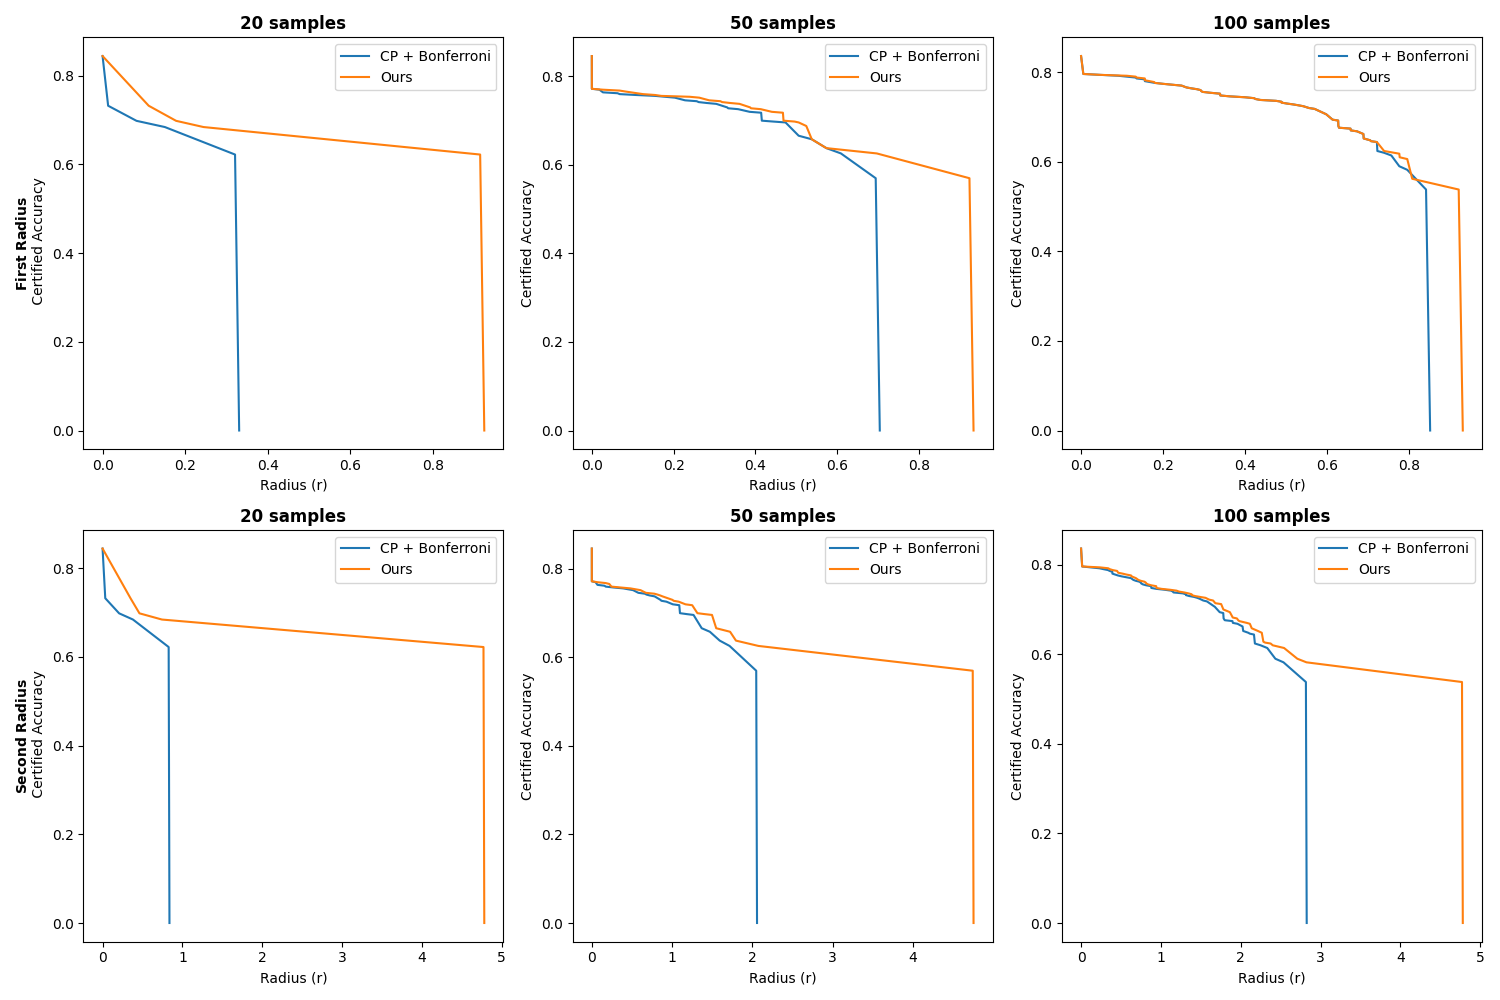
\includegraphics[width=0.8\textwidth]{images/discrete_num}
    \caption{Certified accuracies' comparison on the CIFAR-10 dataset in the discrete case for different numbers of samples (displayed on the columns) with $\sigma = 0.12$. CP + Bonferroni means Clopper-Pearson interval with Bonferroni correction, and dichotomy means our new approach in section~\ref{sec:discrete}. The first row compares the certified accuracies using the first margin and the second row compares the certified accuracies using the second margin.}
    \label{fig:discrete_num}
\end{figure}

\begin{table}[htbp]
    \centering
    \caption{Certified accuracy using the second margin on the CIFAR-10 dataset in the discrete case for different values of radius $r$ with a sample size of $100$ and a standard deviation $\sigma = 0.12$.}
    \label{tab:simplified-certified-accuracy}
    \renewcommand{\arraystretch}{1.2}
    \begin{tabular}{l*{9}{c}}
        \toprule
        Method & \multicolumn{9}{c}{Radius ($r$)} \\
        \cmidrule(l){2-10}
        & 0.5 & 1.0 & 1.5 & 2.0 & 2.5 & 3.0 & 3.5 & 4.0 & 4.5 \\
        \midrule
        CP + Bonferroni & 0.774 & 0.744 & 0.720 & 0.662 & 0.582 & 0.000 & 0.000 & 0.000 & 0.000 \\
        Dichotomy              & 0.780 & 0.746 & 0.726 & 0.670 & 0.614 & 0.538 & 0.538 & 0.538 & 0.538 \\
        Gain (\%) & 0.78\% & 0.27\% & 0.83\% & 1.21\% & 5.50\% & $\infty$ & $\infty$ & $\infty$ & $\infty$ \\
        \bottomrule
    \end{tabular}
\end{table}

The second important hyperparameter is the standard deviation $\sigma$.
As Figure~\ref{fig:discrete_sigma} shows, when the standard deviation increases, the CTA decreases as the classifier’s base accuracy decreases because the added noise makes the classification task harder, leading the model to make more errors on the noisy data.
When the standard deviation is too high, even though the certified radius increases, the base accuracy decreases enough to reduce the overall certified test-set accuracy.
Therefore, the differences between the two methods become more negligible as the standard deviation increases.

\begin{figure}[htbp]
    \centering
    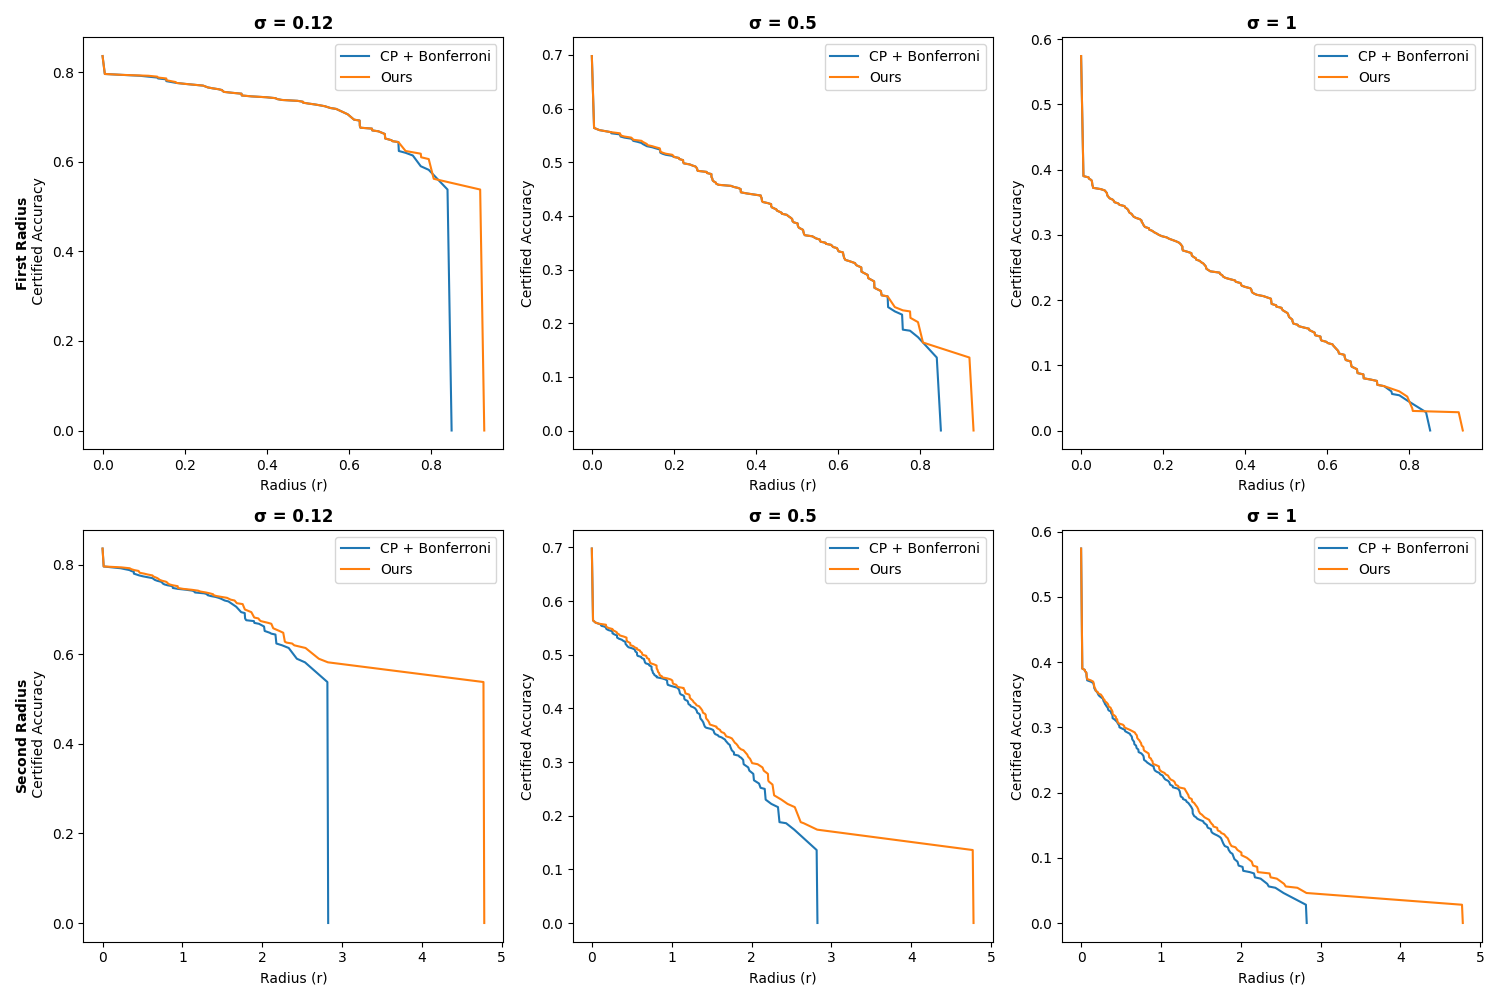
\includegraphics[width=0.8\textwidth]{images/discrete_sigma}
    \caption{Certified accuracies' comparison on the CIFAR-10 dataset in the discrete case for different standard deviations (displayed on the columns) with a sample size of $100$. The legend and row conventions are the same as in Figure~\ref{fig:discrete_num}.}
    \label{fig:discrete_sigma}
\end{figure}

In the continuous case, in addition to the sample size and the standard deviation, another hyperparameter to consider is the \textit{temperature}.
The simplex map $s$ used in the experiments is the tempered softmax function which is a generalization of the standard softmax function, introducing a temperature parameter to control the smoothness of the output distribution.
Given a vector $\mathbf{x} = (x_1, \ldots, x_m)$ and a temperature parameter $T > 0$, the tempered softmax function $\sigma_T: \mathbb{R}^m \to \mathbb{R}^m$ is defined as:
\[
    \sigma_T(\mathbf{x})_i = \frac{\exp(x_i/T)}{\sum_{j=1}^n \exp(x_j/T)}
\]
for $i = 1, \ldots, m$.

As $T \to 0^+$, the tempered softmax approaches a hard maximum (one-hot vector).
As $T \to \infty$, the tempered softmax approaches a uniform distribution.
When $T = 1$, it reduces to the standard softmax function.

Figures~\ref{fig:cont_num} and~\ref{fig:cont_sigma} show the effect of increasing the number of samples $n$ and increasing the standard deviation $\sigma$ respectively.
The effects of these hyperparameters are similar in both discrete and continuous case.
\begin{figure}[htbp]
    \centering
    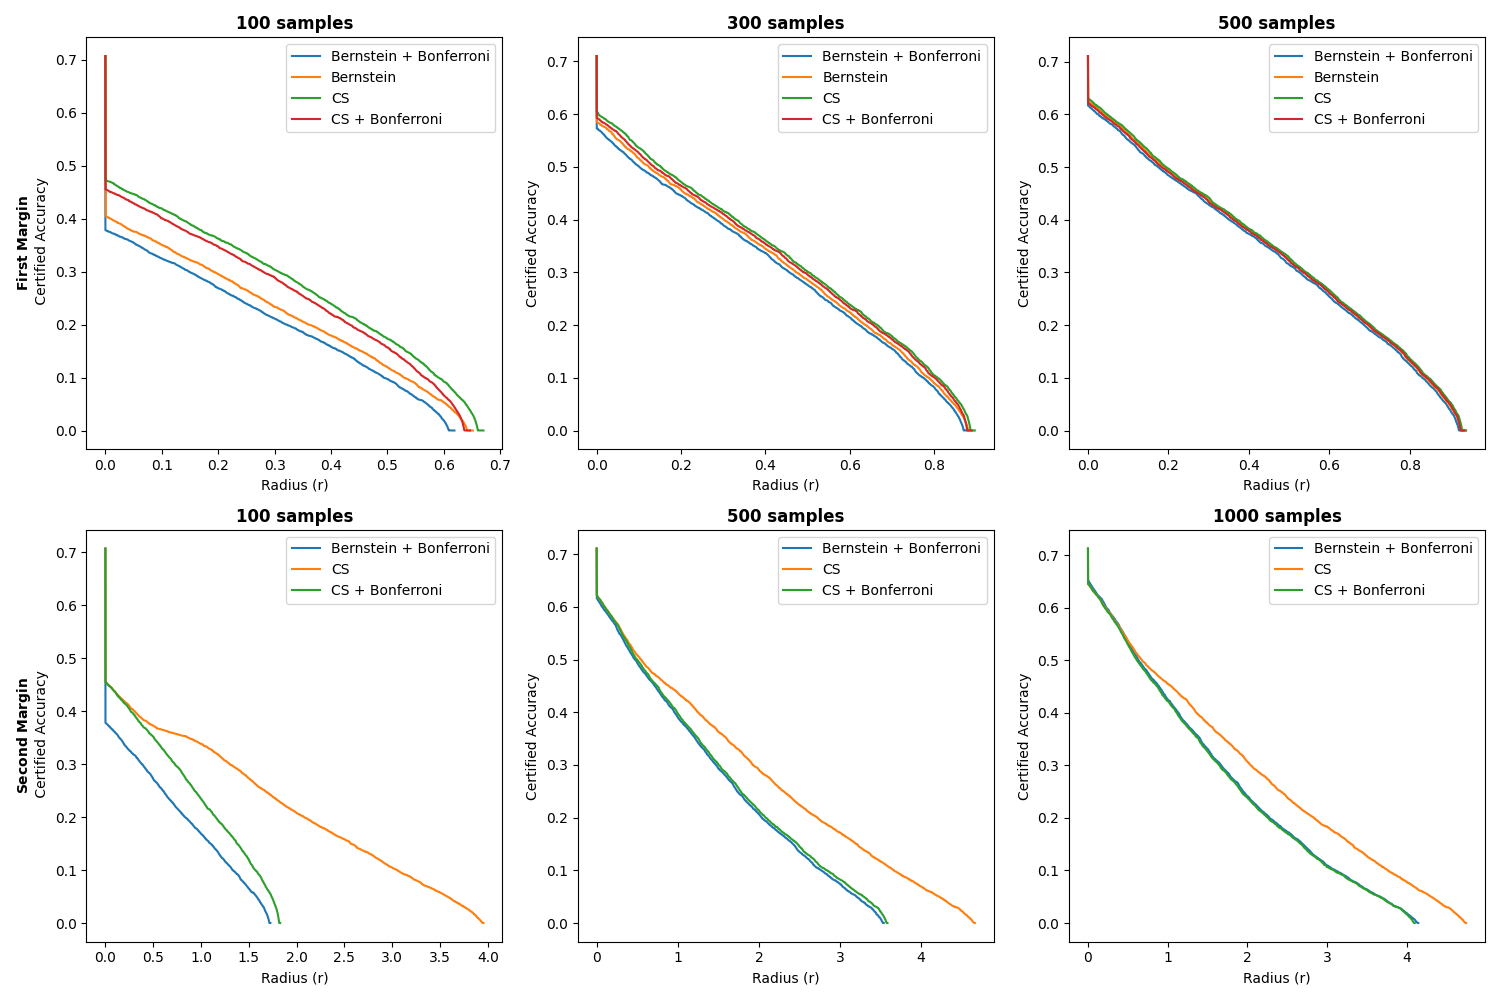
\includegraphics[width=0.8\textwidth]{images/cont_num}
    \caption{Certified accuracies' comparison on the CIFAR-10 dataset in the continuous case for different sample sizes (displayed on the columns) with $\sigma = 0.5$ and a temperature equal to $1$. CS/Bernstein + Bonferroni stands for the Bonferroni approach with either the empirical Bernstein interval (Proposition~\ref{prop:empirical-bernstein-inequality}) or the confidence sequence (Proposition~\ref{prop:confidence-sequence}), and CS/Bernstein stands for the new approach in section~\ref{sec:continuous}. The first row compares the certified accuracies using the first margin and the second row compares the certified accuracies using the second margin.}
    \label{fig:cont_num}
\end{figure}
\begin{figure}[htbp]
    \centering
    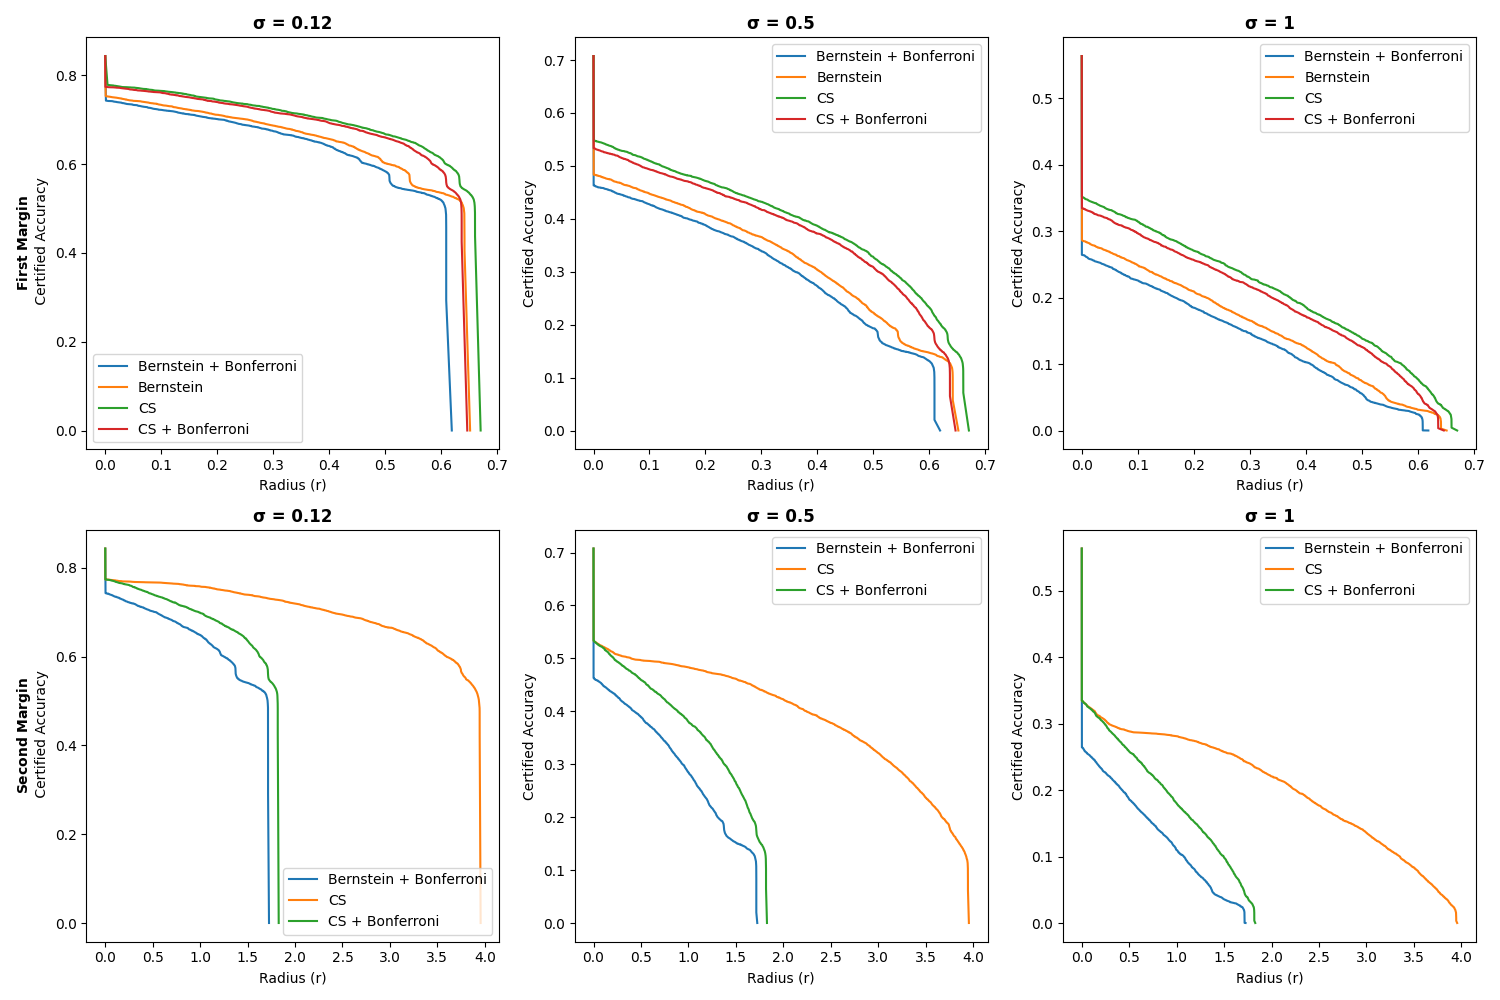
\includegraphics[width=0.8\textwidth]{images/cont_sigma}
    \caption{Certified accuracies' comparison on the CIFAR-10 dataset in the continuous case for different standard deviations (displayed on the columns) with a sample size of $100$ and a temperature equal to $0.1$. The legend and row conventions are the same as in Figure~\ref{fig:cont_num}.}
    \label{fig:cont_sigma}
\end{figure}
\begin{figure}[htbp]
    \centering
    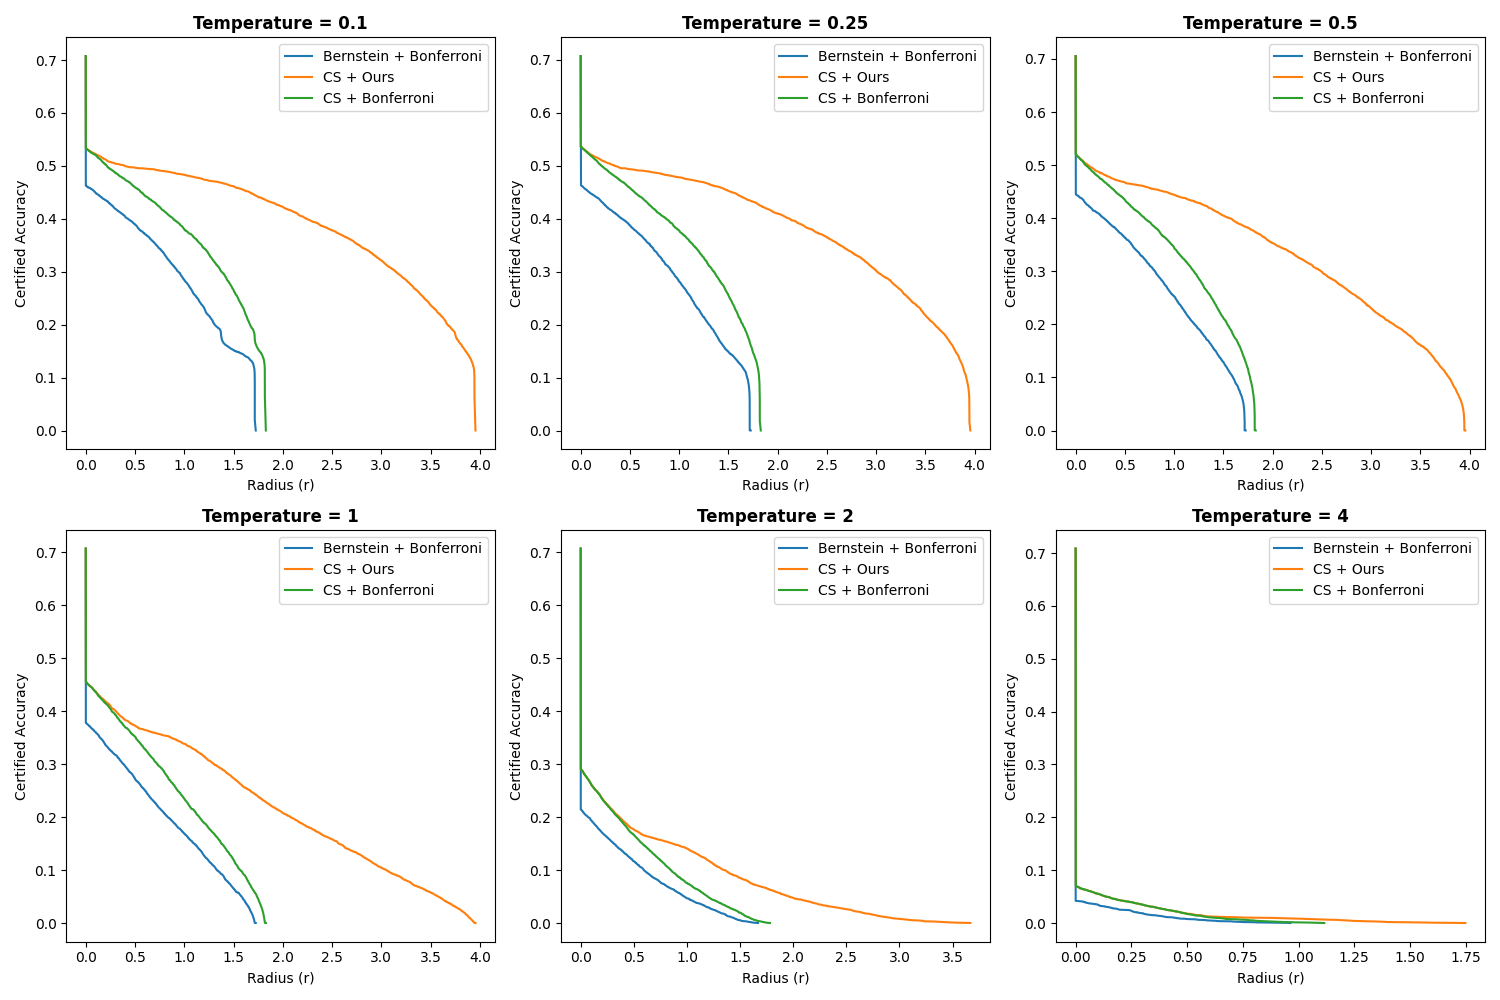
\includegraphics[width=0.8\textwidth]{images/cont_temp}
    \caption{Certified accuracies' comparison on the CIFAR-10 dataset in the continuous case for different temperatures (displayed on the columns) with a sample size of $100$ and $\sigma = 0.5$. The legend and row conventions are the same as in Figure~\ref{fig:cont_num}.}
    \label{fig:cont_temp}
\end{figure}

\begin{table}[htbp]
    \centering
    \caption{Certified accuracy using the first margin on CIFAR-10 in the continuous case for different values of radius $r$ and sample sizes with $\sigma = 0.5$ and a temperature of $1$.}
    \label{tab:certified-accuracy}
    \renewcommand{\arraystretch}{1.2}
    \begin{tabular}{@{}ll*{9}{c}@{}}
        \toprule
        \multirow{2}{*}{Samples} & \multirow{2}{*}{Method} & \multicolumn{9}{c}{Radius ($r$)} \\
        \cmidrule(l){3-11}
        & & 0.1 & 0.2 & 0.3 & 0.4 & 0.5 & 0.6 & 0.7 & 0.8 & 0.9 \\
        \midrule
        \multirow{3}{*}{100}
        & CS + Bonferroni & 0.400 & 0.347 & 0.289 & 0.220 & 0.157 & 0.066 & 0.000 & 0.000 & 0.000 \\
        & CS              & 0.419 & 0.362 & 0.303 & 0.239 & 0.173 & 0.092 & 0.000 & 0.000 & 0.000 \\
        & Comparison (\%) & 4.69\% & 4.28\% & 5.04\% & 8.70\% & 10.65\% & 39.16\% & N/A & N/A & N/A \\
        \midrule
        \multirow{3}{*}{300}
        & CS + Bonferroni & 0.526 & 0.464 & 0.411 & 0.354 & 0.296 & 0.233 & 0.173 & 0.101 & 0.000 \\
        & CS              & 0.536 & 0.471 & 0.416 & 0.361 & 0.301 & 0.239 & 0.179 & 0.105 & 0.000 \\
        & Comparison (\%) & 1.93\% & 1.55\% & 1.39\% & 1.89\% & 1.94\% & 2.52\% & 3.49\% & 4.06\% & N/A \\
        \midrule
        \multirow{3}{*}{500}
        & CS + Bonferroni & 0.560 & 0.490 & 0.434 & 0.379 & 0.322 & 0.261 & 0.199 & 0.133 & 0.050 \\
        & CS              & 0.568 & 0.497 & 0.442 & 0.383 & 0.329 & 0.266 & 0.202 & 0.136 & 0.054 \\
        & Comparison (\%) & 1.43\% & 1.33\% & 2.00\% & 0.99\% & 2.08\% & 2.01\% & 1.89\% & 2.33\% & 9.21\% \\
        \bottomrule
    \end{tabular}
\end{table}
\begin{table}[htbp]
    \centering
    \caption{Certified accuracy using the second margin on CIFAR-10 in the continuous case for different values of radius $r$ and sample sizes with $\sigma = 0.5$ and a temperature of $1$.}
    \label{tab:certified-accuracy-2}
    \renewcommand{\arraystretch}{1.2}
    \begin{tabular}{@{}ll*{9}{c}@{}}
        \toprule
        \multirow{2}{*}{Samples} & \multirow{2}{*}{Method} & \multicolumn{9}{c}{Radius ($r$)} \\
        \cmidrule(l){3-11}
        & & 0.1 & 0.2 & 0.3 & 0.4 & 0.5 & 0.6 & 0.7 & 0.8 & 0.9 \\
        \midrule
        \multirow{3}{*}{100}
        & CS + Bonferroni & 0.436 & 0.415 & 0.393 & 0.369 & 0.352 & 0.328 & 0.305 & 0.284 & 0.259 \\
        & CS              & 0.437 & 0.418 & 0.401 & 0.383 & 0.373 & 0.364 & 0.359 & 0.354 & 0.347 \\
        & Comparison (\%) & 0.19\% & 0.83\% & 1.91\% & 3.72\% & 5.95\% & 11.17\% & 17.68\% & 24.67\% & 34.03\% \\
        \midrule
        \multirow{3}{*}{300}
        & CS + Bonferroni & 0.572 & 0.545 & 0.518 & 0.493 & 0.471 & 0.451 & 0.431 & 0.413 & 0.391 \\
        & CS              & 0.572 & 0.547 & 0.523 & 0.500 & 0.481 & 0.465 & 0.451 & 0.439 & 0.427 \\
        & Comparison (\%) & 0.00\% & 0.42\% & 0.92\% & 1.46\% & 2.15\% & 2.97\% & 4.59\% & 6.25\% & 9.24\% \\
        \midrule
        \multirow{3}{*}{500}
        & CS + Bonferroni & 0.600 & 0.578 & 0.553 & 0.525 & 0.500 & 0.478 & 0.457 & 0.437 & 0.419 \\
        & CS              & 0.600 & 0.578 & 0.556 & 0.530 & 0.509 & 0.489 & 0.473 & 0.461 & 0.448 \\
        & Comparison (\%) & 0.08\% & 0.08\% & 0.53\% & 1.03\% & 1.77\% & 2.29\% & 3.50\% & 5.62\% & 6.98\% \\
        \bottomrule
    \end{tabular}
\end{table}

It is clear from Figure~\ref{fig:cont_temp} that increasing the temperature parameter $T$ reduces the discrepancies between the Bonferroni approach and our new method.
Higher temperatures lead to softer decision boundaries.
As the temperature increases, the output probabilities of the tempered softmax function become more uniform, regardless of the input values.
This means that the function becomes less sensitive to differences in the input, causing different methods to produce more similar outputs.
Hence, as the temperature rises, the tempered softmax function becomes less responsive to changes in its inputs.
This means that larger changes in the input are required to produce the same change in output probabilities.
Consequently, the differences between various methods become less pronounced.
At lower temperatures, the tempered softmax accentuates differences between inputs.
The highest value tends to dominate, resulting in an output distribution that's closer to a one-hot vector.


    \section{Conclusion and Future Work}\label{sec:conclusion-and-future-work}
In this paper, we have presented novel techniques for improving the estimation of certified radii in randomized smoothing, leading to tighter bounds on certified test-set accuracy.
Our methods have demonstrated significant improvements on both CIFAR-10 and ImageNet datasets, showcasing the potential for more efficient and accurate certification of neural network robustness against adversarial perturbations.
While our results mark a substantial step forward in the field of adversarial robustness, they also open up several promising avenues for future research:
One particularly intriguing direction is the development of more efficient tricks for estimating certified radii in discrete domains.
In the continuous case, our work has highlighted the importance of tight confidence intervals for accurate estimation of certified radii, leaving the exploration of tighter confidence sequences and the development of new theoretical frameworks that provide rigorous backing for the tightness of these improved confidence intervals for future work.
By pursuing these lines of research, we hope to further narrow the gap between empirical performance and theoretical guarantees in randomized smoothing.
We leave for future the comparison between empirical certified radii (like those based on PGD attacks) and estimated certified radii.


    \section*{Acknowledgments}
This work on randomized smoothing would not have been possible without the guidance, support, and expertise of several individuals to whom I am deeply grateful.

First and foremost, I would like to express my sincere gratitude to my internship mentor, Blaise Delattre, for his thought-provoking questions and constructive feedback, which have pushed me to think more critically about the implications and applications of our work, and for his meticulous attention to detail has undoubtedly improved the quality of this work and helped me formulate more rigorous proofs for our proposed methods.
His patient guidance, insightful discussions, and unwavering support have been instrumental in shaping this research.

I am also indebted to Dr. Paul Caillon and Pr. Alexandre Allauzen, for their profound knowledge of adversarial robustness and machine learning and for their insightful remarks and recommendations during all the stages of this project.
Their broad perspective on the field of machine learning security and general advice on research methodology have been invaluable in shaping the direction of this work and elevating the quality and relevance of our contributions.

Special Thanks to Erwan Fagnou for his help on the implementation of the code of this paper.

I would like to thank the PRAIRIE institute for this invaluable internship opportunity.

This experience has been invaluable for my academic and professional growth, and I am truly thankful for the opportunity to work with such exceptional mentors and colleagues in the field of randomized smoothing and adversarial robustness.


    \appendix

    \section{Signomial Programming}\label{sec:signomial-programming}

\subsection{Definitions}\label{subsec:definitions}
In signomial programming, the building block is a \textbf{monomial} function which is a function of the form
\[f(\mathbf{x}) = c x_1^{a_1} x_2^{a_2} \cdots x_m^{a_m}\]

where:
\begin{itemize}
    \item $c > 0$ is a positive coefficient,
    \item $\mathbf{x} = (x_1, x_2, \ldots, x_m)$ are positive variables,
    \item $a_1, a_2, \ldots, a_m$ are real exponents (not necessarily non-negative).
\end{itemize}
Building on top of this definition, we can define two types of functions.
A \textbf{posynomial} function is a sum of monomials, while a \textbf{signomial} function is a linear combination of monomials (meaning that the multiplicative coefficients can be negative).

A signomial program (SP) is an optimization problem of the form:
\[
    \begin{aligned}
        & \text{minimize}   & & f_0(\mathbf{x}) \\
        & \text{subject to} & & f_i(\mathbf{x}) \geq 0, \quad i = 1, \ldots, p \\
        &                   & & \mathbf{x} > 0
    \end{aligned}
\]
where:

\begin{itemize}
    \item $\mathbf{x} = (x_1, \ldots, x_m)$ is the vector of optimization variables,
    \item $f_0, f_1, \ldots, f_m$ are signomial functions.
\end{itemize}

Signomials programs generalize the well-known geometric programs that are much easier to solve, since they can be reduced to convex optimization problems.
However, signomial programs are generally non-convex optimization problems and can be challenging to solve globally.
Various techniques, such as successive convex approximation or branch-and-bound methods, are often employed to find solutions to SPs.



    \section{Proofs}\label{sec:proofs}

\subsection{Proof of Lemma \ref{lemma:suboptimal}}\label{subsec:proof-of-lemma-ref{lemma:suboptimal}}
\begin{proof}
    Suppose there exists $q^0\in\Delta^{2}$ such that $q^0_1-q^0_2\leq L$ and $\Pi(\Tilde{\theta}|q^0)\leq 1-\alpha$ for some $L\in\Theta$.
    It follows that
    \[
        \inf_{\substack{q\in\Delta^{2}\\q_1-q_2\leq L}}\Pi(\Tilde{\theta}|q)\leq\Pi(\Tilde{\theta}|q^0)\leq 1-\alpha.
    \]
    In other terms,
    \[\alpha\leq\Pi(L).\]
    Since $\Pi$ is nondecreasing, by definition of $\underline{\Hat{\theta}}$,
    \[\Pi(\underline{\Hat{\theta}})\leq\alpha.\]
    Therefore, $\Pi(\underline{\Hat{\theta}})\leq\Pi(L)$, which implies $\underline{\Hat{\theta}}\leq L$.
\end{proof}

\subsection{Proof of Lemma \ref{lemma:approximation}}\label{subsec:proof-of-lemma-ref{lemma:approximation}}
\begin{proof}
    To recall, the error function, denoted as $\text{erf}(x)$, is defined as

    \[
        \text{erf}(x) = \frac{2}{\sqrt{\pi}} \int_0^x e^{-t^2} dt.
    \]

    Its domain of the error function is the interval $(-\infty, \infty)$, and its codomain is the interval $(-1, 1)$.
    The error function is an increasing and odd function.

    The inverse error function, denoted as $\text{erf}^{-1}(z)$, is the inverse of the error function.
    Its domain is the interval $(-1, 1)$, and its codomain is all real numbers.
    Due to the complexity of the error function, the inverse error function does not have a simple closed-form expression.
    However, it can be approximated using various methods.

    One such approximation for the inverse error function is given by the following series:

    \[
        \text{erf}^{-1}(x) = \sum_{k=0}^{\infty} \frac{c_k}{2k+1} \left(\frac{\sqrt{\pi}}{2}x\right)^{2k+1}
    \]

    where $c_0 = 1$ and the subsequent coefficients $c_k$ are defined recursively as:

    \[
        c_k = \sum_{m=0}^{k-1} \frac{c_m c_{k-1-m}}{(m+1)(2m+1)}.
    \]

    This series approximation converges on the entire domain of the inverse error function.
    If we denote by $\text{erf}_M$ the $M$-th order Taylor series of the error function,
    \[
        \text{erf}_M(x) \coloneqq \sum_{k=0}^M \frac{c_k}{2k+1} \left(\frac{\sqrt{\pi}}{2}x\right)^{2k+1},
    \]
    then it is clear that $\text{erf}(x) \geq\text{erf}_M(x)$ if $x\geq0$, and $\text{erf}(x) \leq\text{erf}_M(x)$ otherwise.

    The Gaussian quantile function, denoted as $\Phi^{-1}$, can be expressed in terms of the inverse error function as follows
    \[\Phi^{-1}(p) = \sqrt{2} \cdot \text{erf}^{-1}(2p - 1).\]

    The domain of $\Phi^{-1}(p)$ is $(0, 1)$, corresponding to probabilities, while its codomain is $\mathbb{R}$.
    The Taylor series approximation of $\text{erf}^{-1}(x)$ naturally leads to an approximation of the Gaussian quantile function.
    By substituting $x = 2p - 1$ into the Taylor series for $\text{erf}^{-1}(x)$ and multiplying by $\sqrt{2}$, we obtain
    \[\Phi^{-1}(p) \approx \sqrt{2} \sum_{k=0}^{M} \frac{c_k}{2k+1} \left(\frac{\sqrt{\pi}}{2}(2p-1)\right)^{2k+1}\coloneqq\Phi^{-1}_M(p)\]
    It follows that if $p\geq\frac{1}{2}$, then $\Phi^{-1}(p) \geq\Phi^{-1}_M(p)$, and if $p\leq\frac{1}{2}$, then $\Phi^{-1}(p) \leq\Phi^{-1}_M(p)$, which concludes the proof.
\end{proof}

    \section{More Experimental Results}\label{sec:more-experimental-results}
We conducted our experiments on the ImageNet dataset in the same way as in Section~\ref{sec:results}.
The only difference is that we used a 50-layer residual network instead of the 110-layer one.
The figures of the Imagenet dataset are consistent with our previous findings on the CIFAR-10 dataset.
\begin{figure}[htbp]
    \centering
    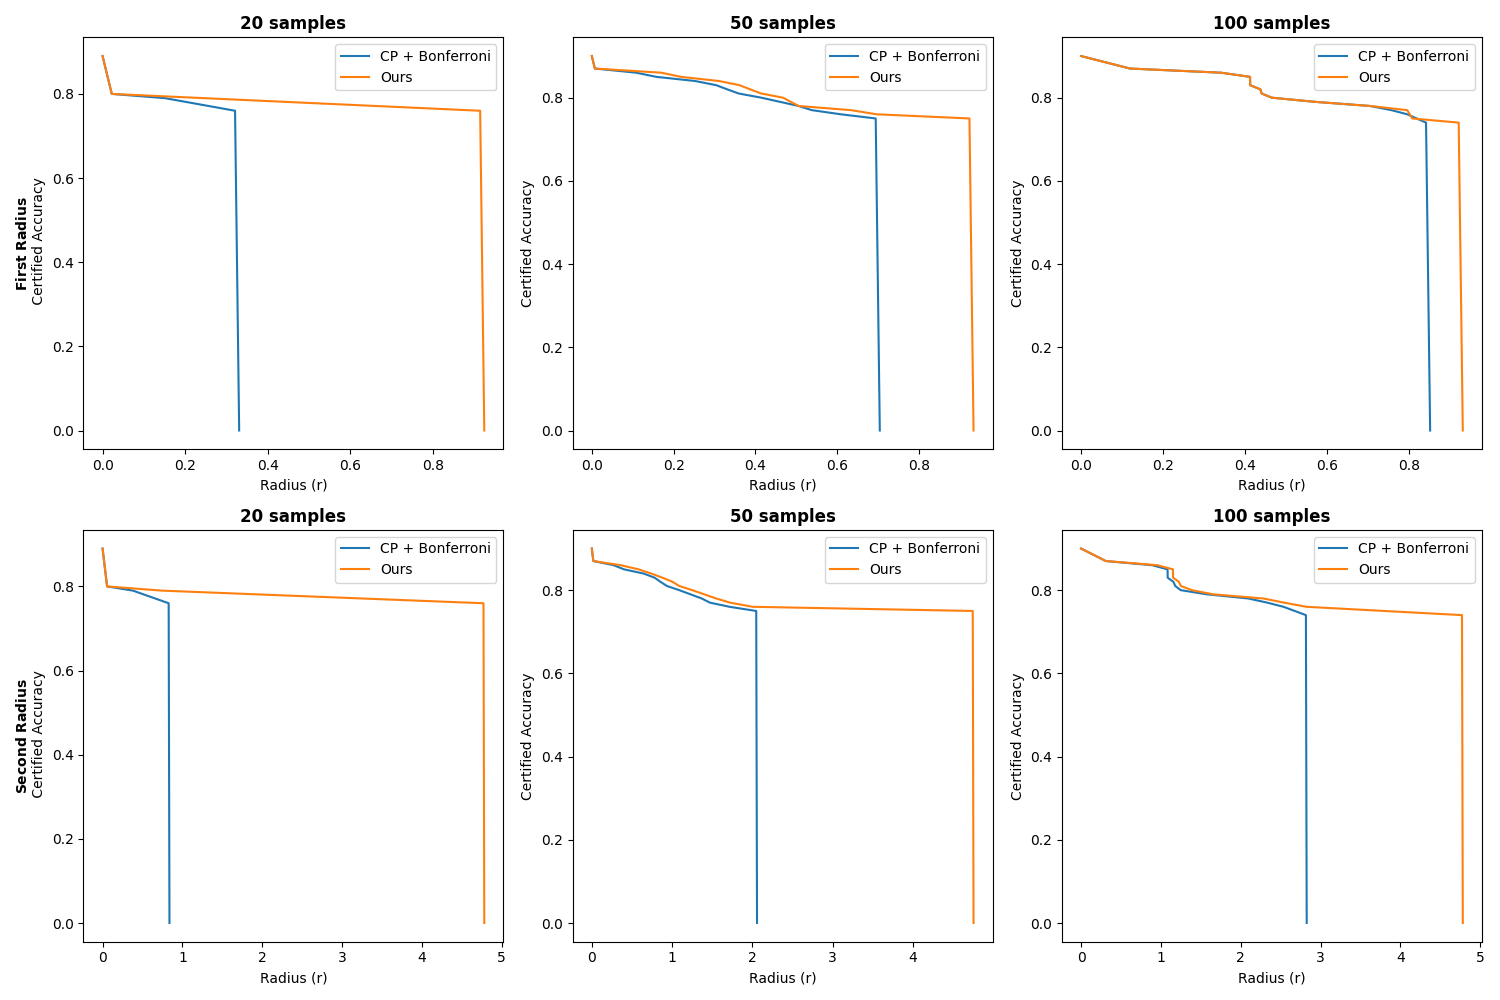
\includegraphics[width=0.8\textwidth]{images/discrete_num_imagenet}
    \caption{Caption for the figure.}
    \label{fig:discrete_num_imagenet}
\end{figure}
\begin{figure}[htbp]
    \centering
    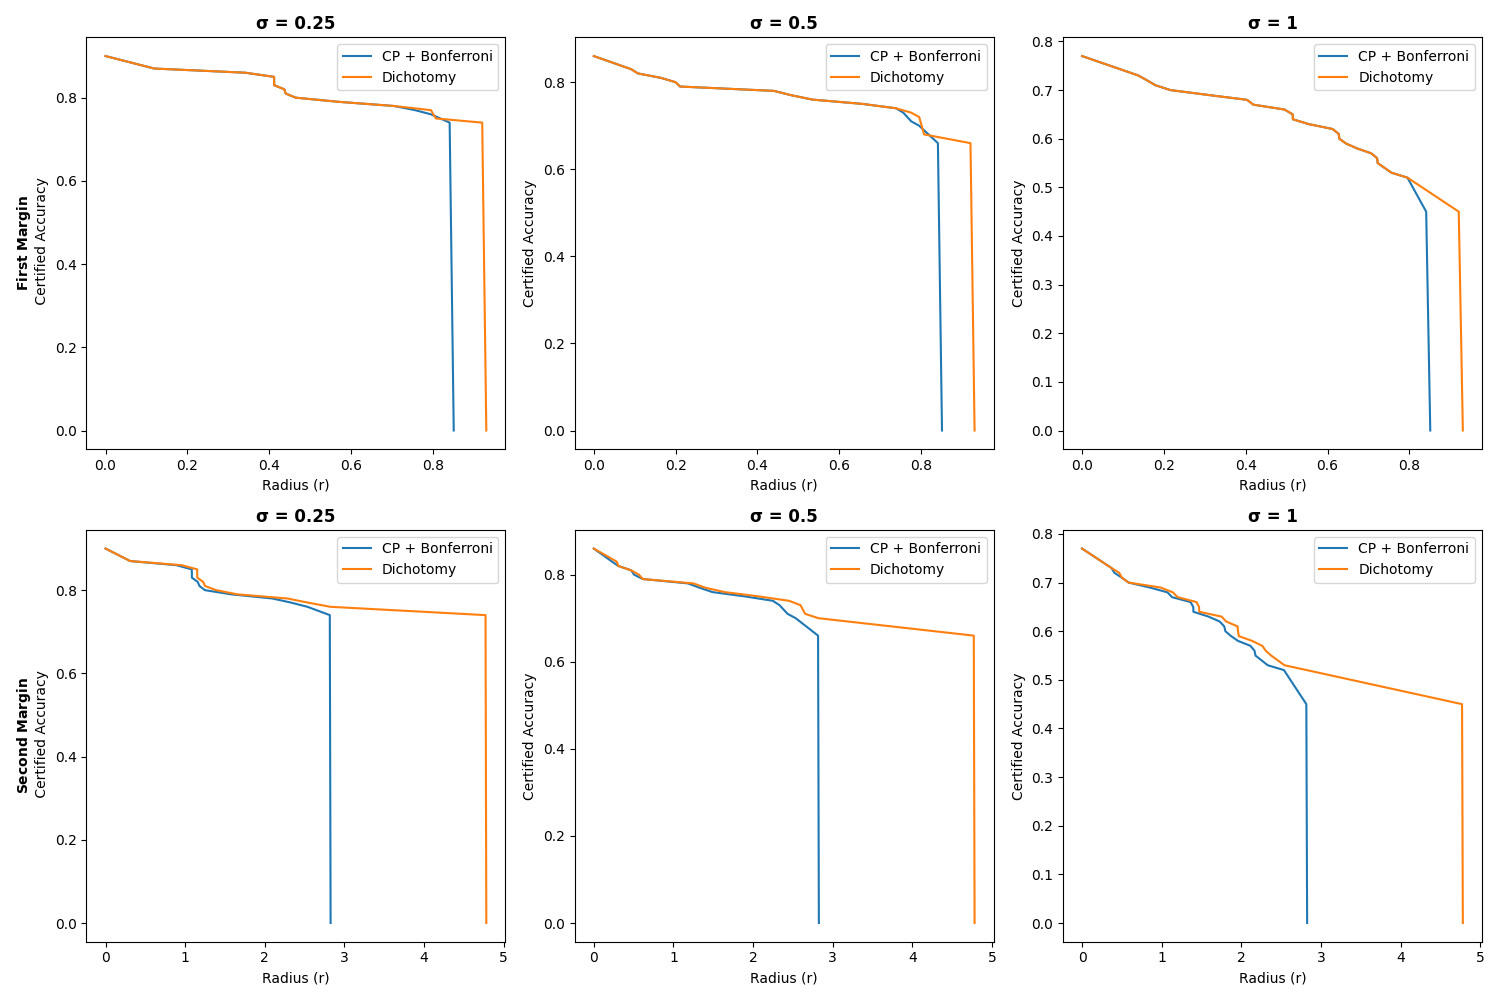
\includegraphics[width=0.8\textwidth]{images/discrete_sigma_imagenet}`
    \caption{Caption for the figure.}
    \label{fig:discrete_sigma_imagenet}
\end{figure}
\begin{figure}[htbp]
    \centering
    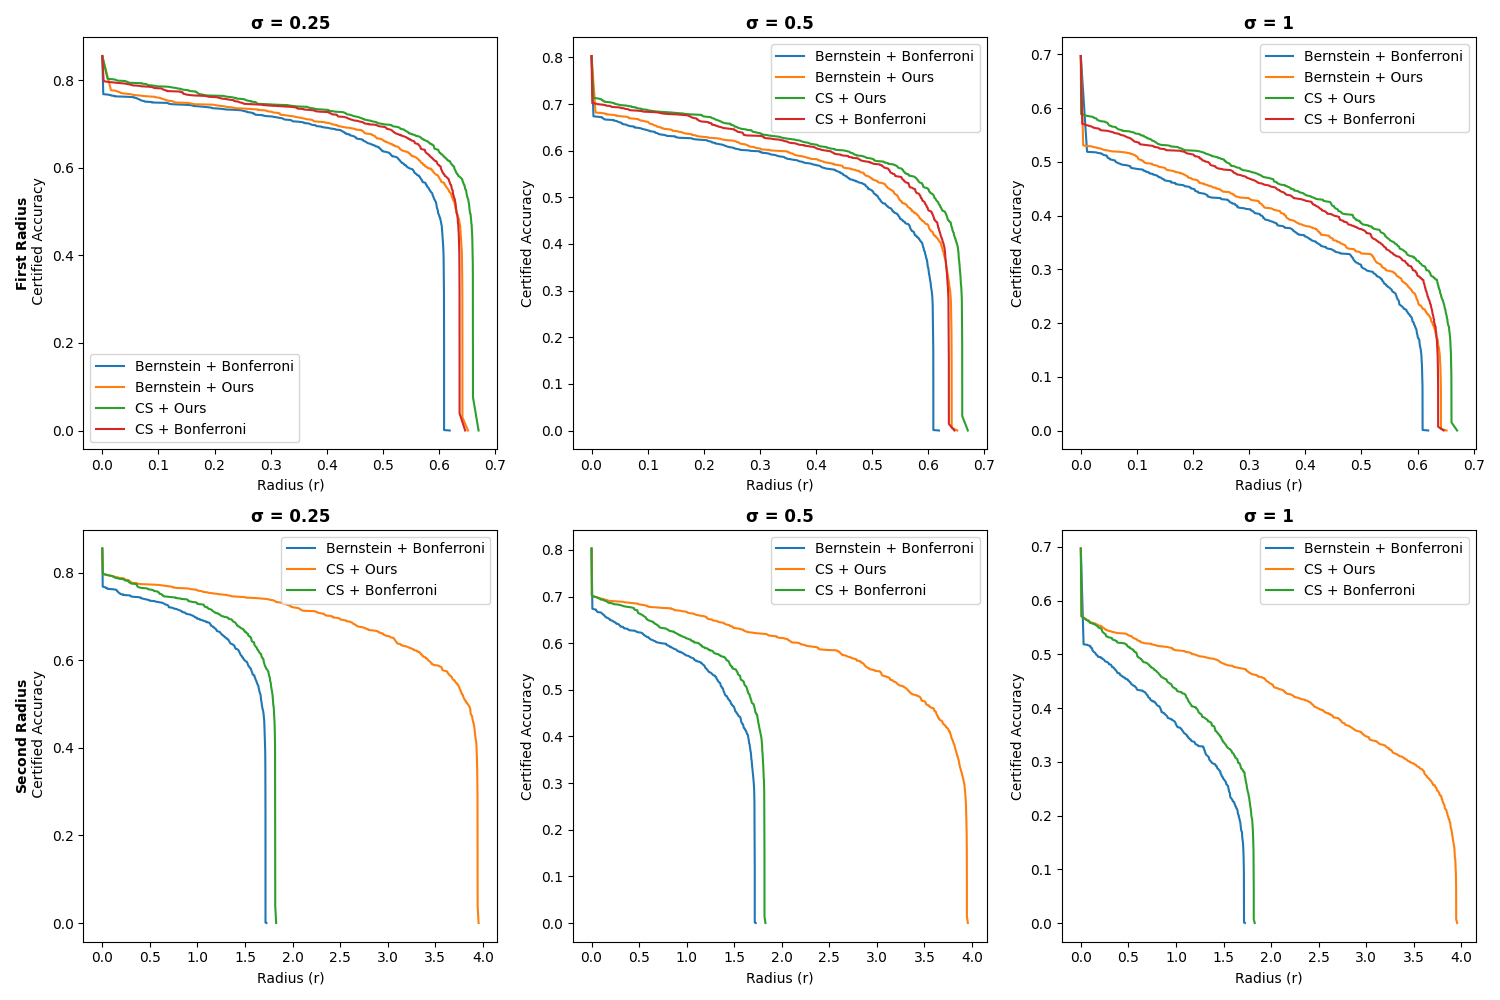
\includegraphics[width=0.8\textwidth]{images/cont_sigma_imagenet}`
    \caption{Caption for the figure.}
    \label{fig:cont_sigma_imagenet}
\end{figure}
\begin{figure}[htbp]
    \centering
    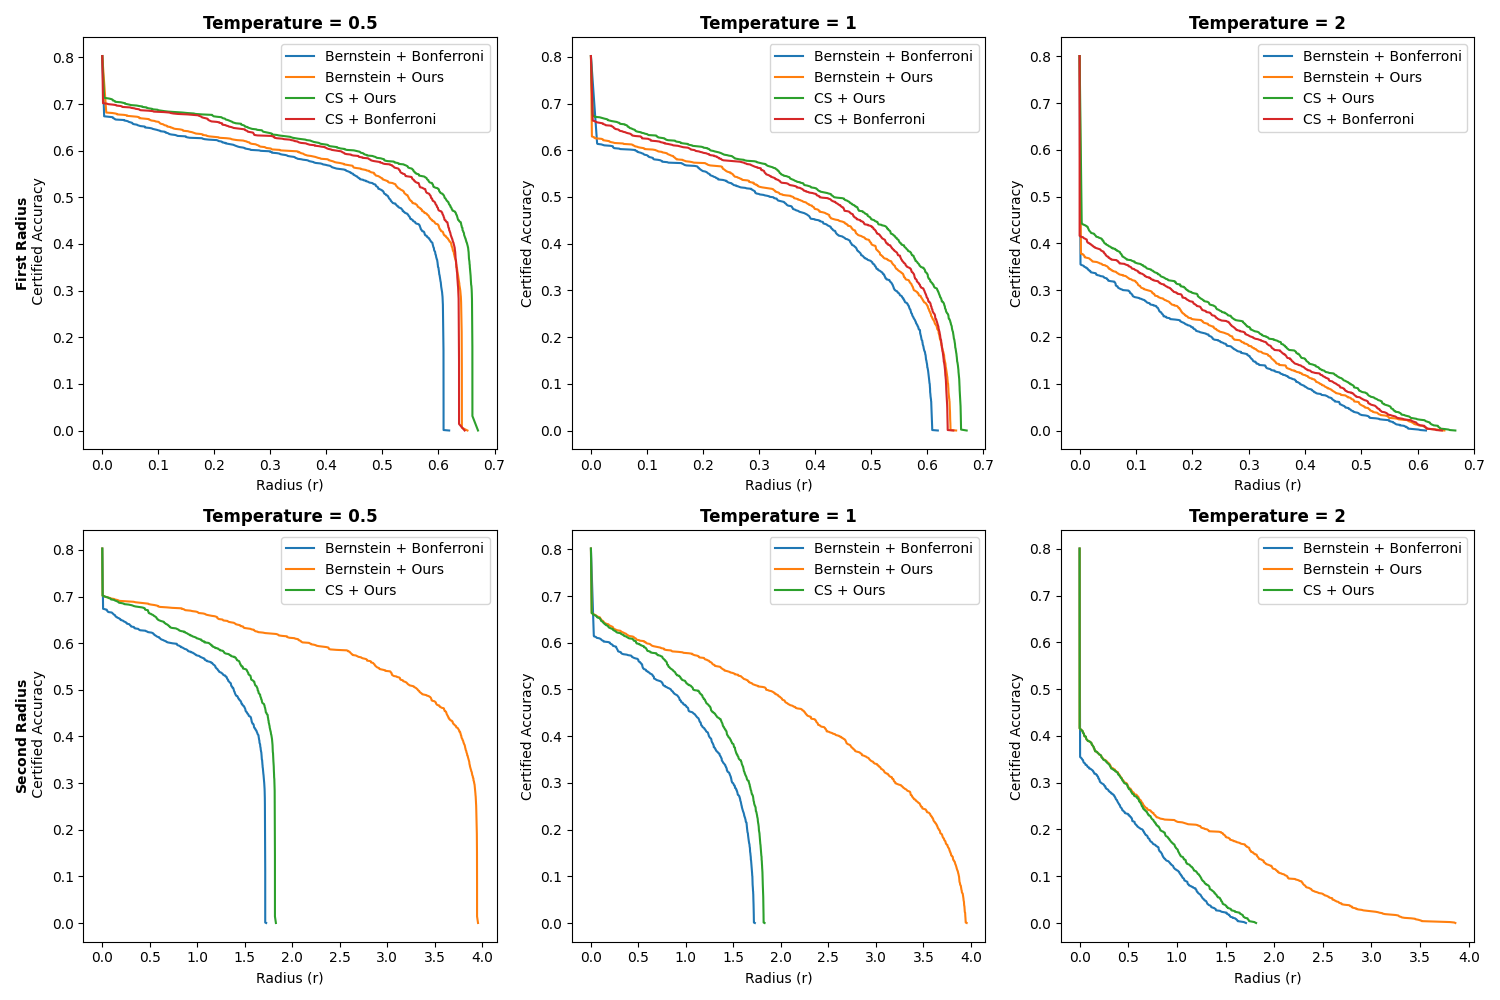
\includegraphics[width=0.8\textwidth]{images/cont_temp_imagenet}
    \caption{Caption for the figure.}
    \label{fig:cont_temp_imagenet}
\end{figure}


    % Bibliography
%    \bibliographystyle{plainnat} % Changed from unsrt to plainnat
    \bibliographystyle{apalike}
    \bibliography{references}


\end{document}
